\documentclass[12pt]{article}
\usepackage{mathtools}
\usepackage{mdframed}
\usepackage{fullpage}
\usepackage{amsfonts}
\usepackage{tikz}
\usepackage{fancyhdr}
\usepackage{lastpage}
\usepackage{graphicx}
\usepackage{subfig}

\graphicspath{{engl314/instructional/}}


%edit this for each class
\newcommand\name{How to fold a paper plane}
\newcommand\head[1]{\noindent{\large\textbf{#1}}:\newline}

\pagestyle{fancy}
\rfoot{\name, page \thepage/\pageref{LastPage}}
\cfoot{}
\rhead{}
\lhead{}
\renewcommand{\headrulewidth}{0pt}
\renewcommand{\footrulewidth}{0pt}

\makeatletter
\renewcommand{\fnum@figure}{\textbf{Step \thefigure}}
\makeatother

\title{How to Fold a Paper Airplane}
\author{Group XXDF}

\fontfamily{helvet}

\footnotetext[1]{ Paper airplane is in no way stealthy and will not actually hide your secret messages.
If you throw this plane in a lecture hall or classroom your instructor will see it, and will confiscate it.
No patent exists for paper airplane design. \label{fnt1}}


\begin{document}
\maketitle\thispagestyle{fancy}

\head{Introduction}
\indent Have you ever wanted to send super secret messages across the classroom or lecture hall that no one else was allowed to read? Well, with our patented
stealth paper plane design you can\footnotemark[\ref{fnt1}]! Watch as your stealth plane soars across the skies of your lecture hall.\\

\head{Materials}
\indent One sheet of $8\frac{1}{2}''\times 11''$ paper\\
\indent Colored pencils (optional)\\

\head{Instructions}
\begin{figure}[h]
  \centering
  \caption{Fold the paper in half vertically (hotdog style).}
  \subfloat{{\includegraphics[width=0.33\textwidth]{engl314/instructional/images/first.png} }}
  \qquad
  \subfloat{{\includegraphics[width=.375\textwidth]{engl314/instructional/images/second.png} }}
\end{figure}
\clearpage


\begin{figure}[!t]
  \centering
  \caption{Fold each top corner into the center fold.}
  \subfloat{{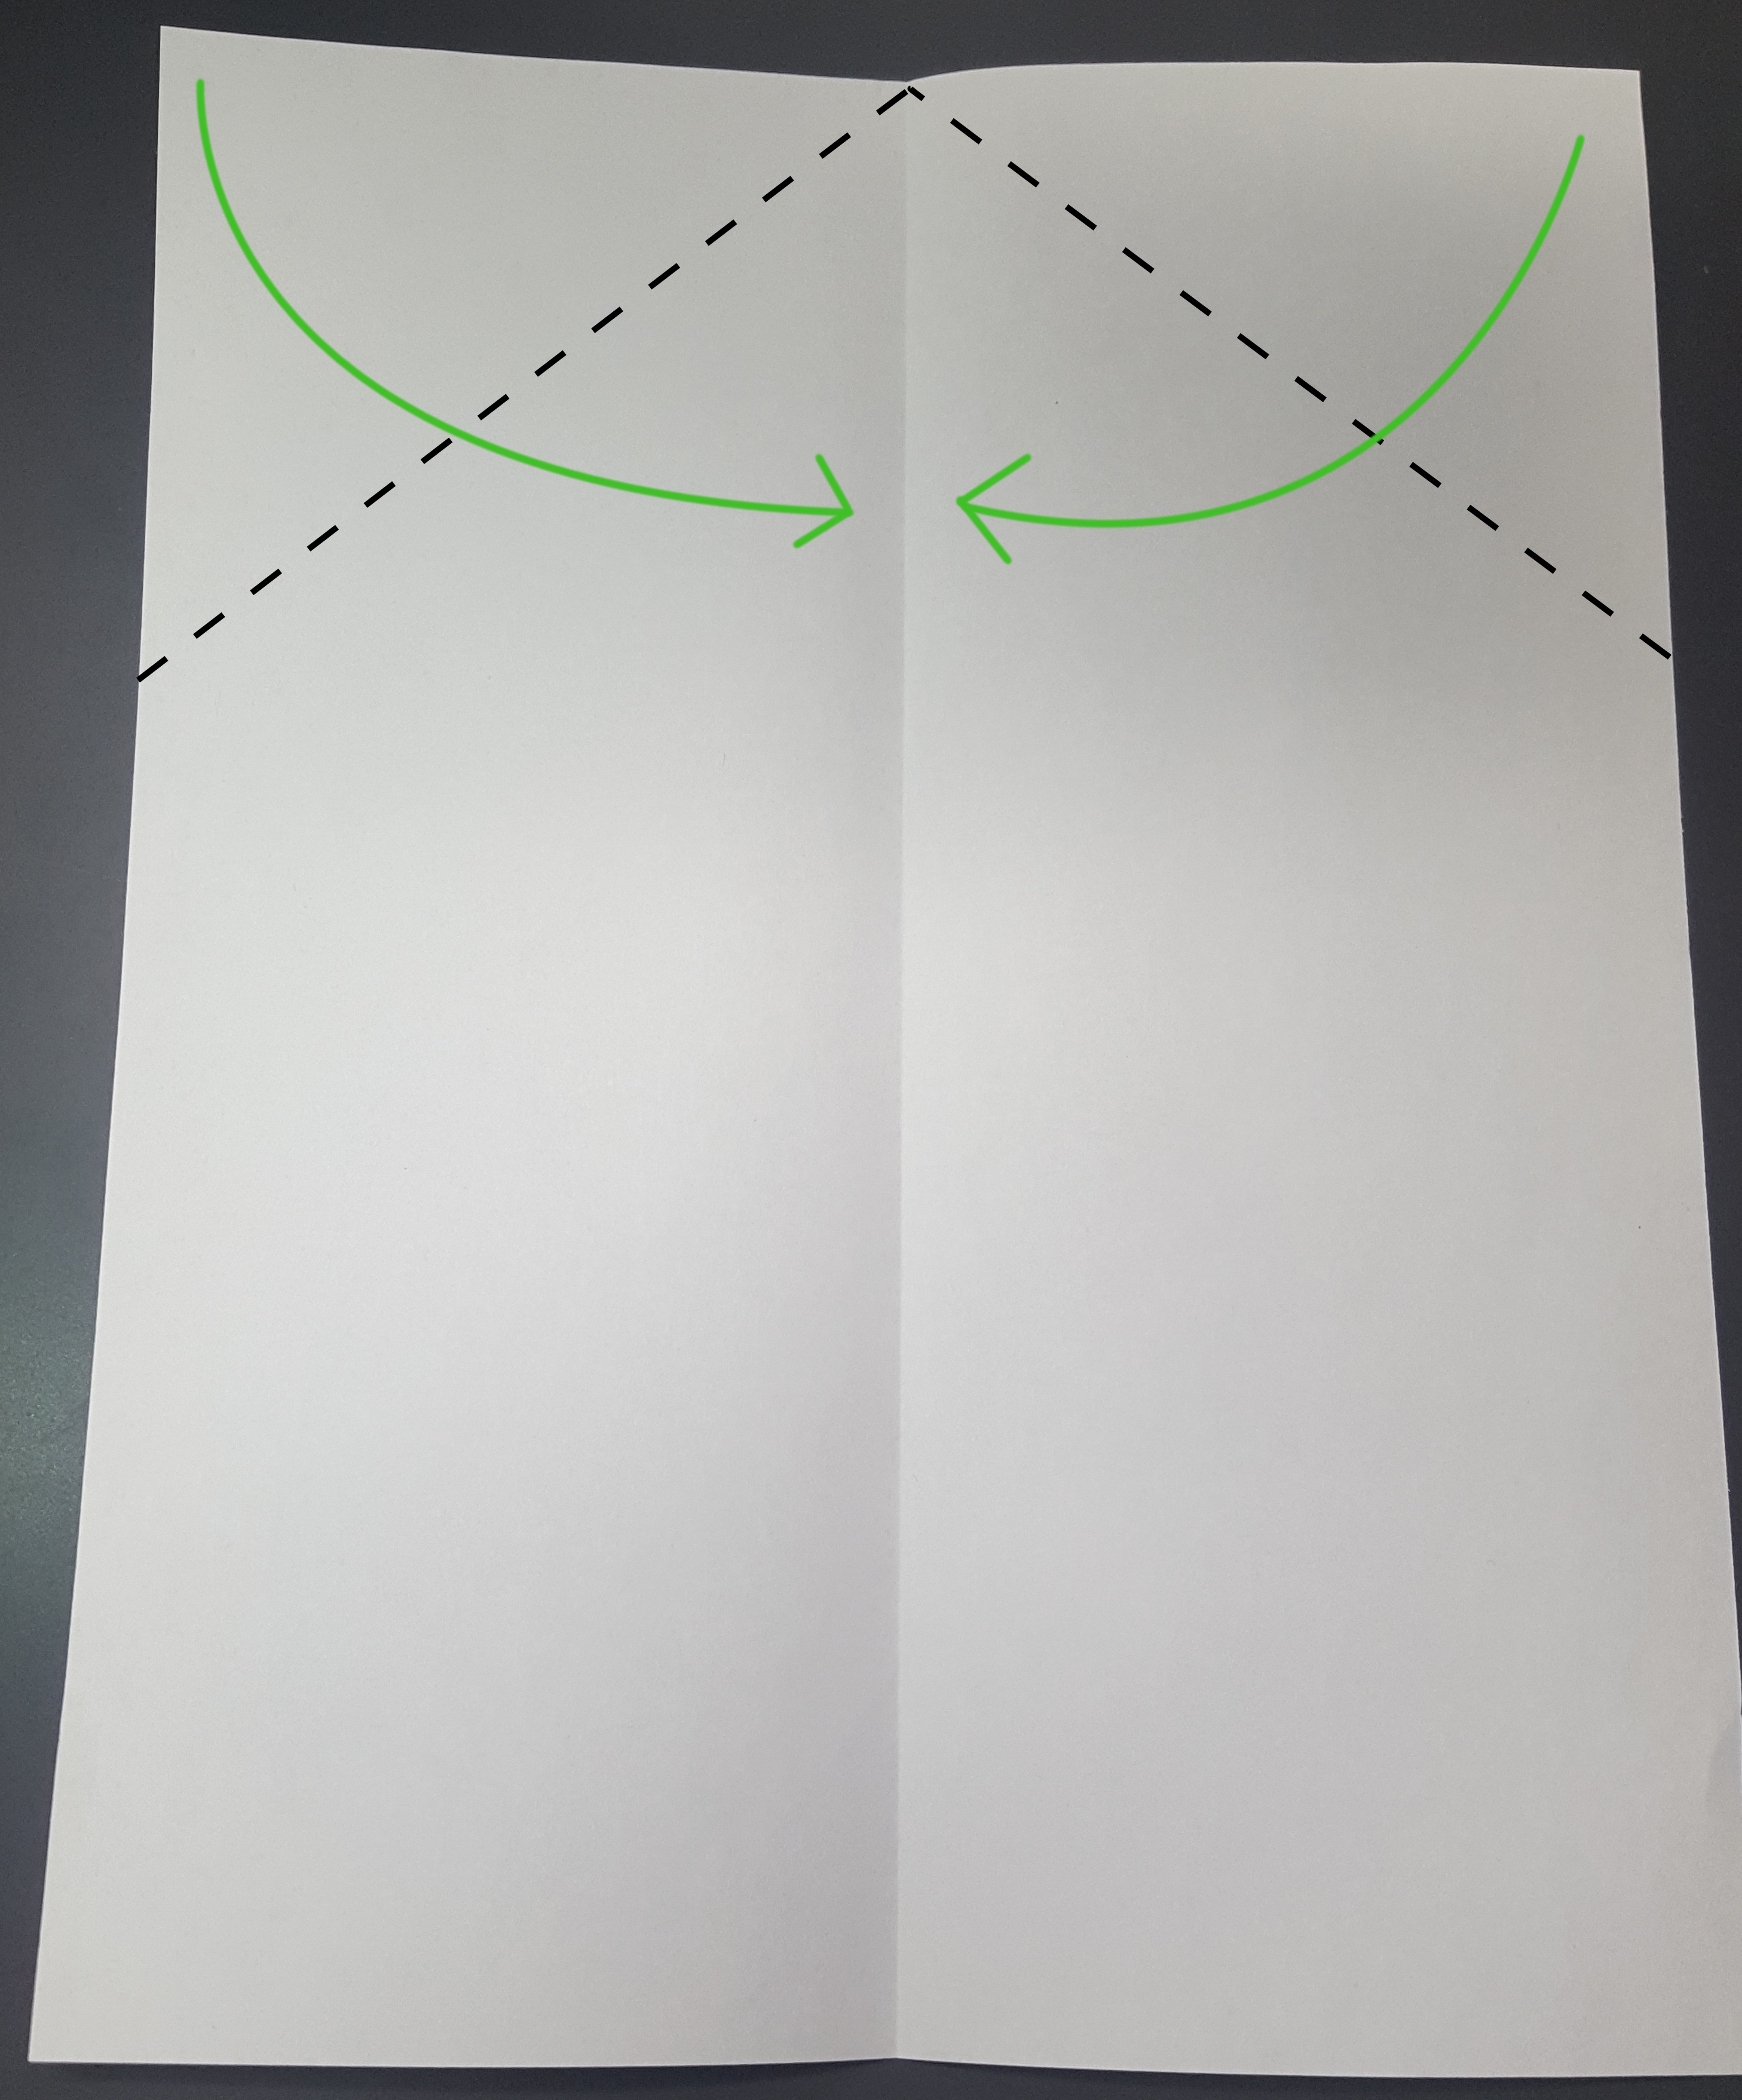
\includegraphics[width=0.4\textwidth]{engl314/instructional/images/third.jpg} }}
  \qquad
  \subfloat{{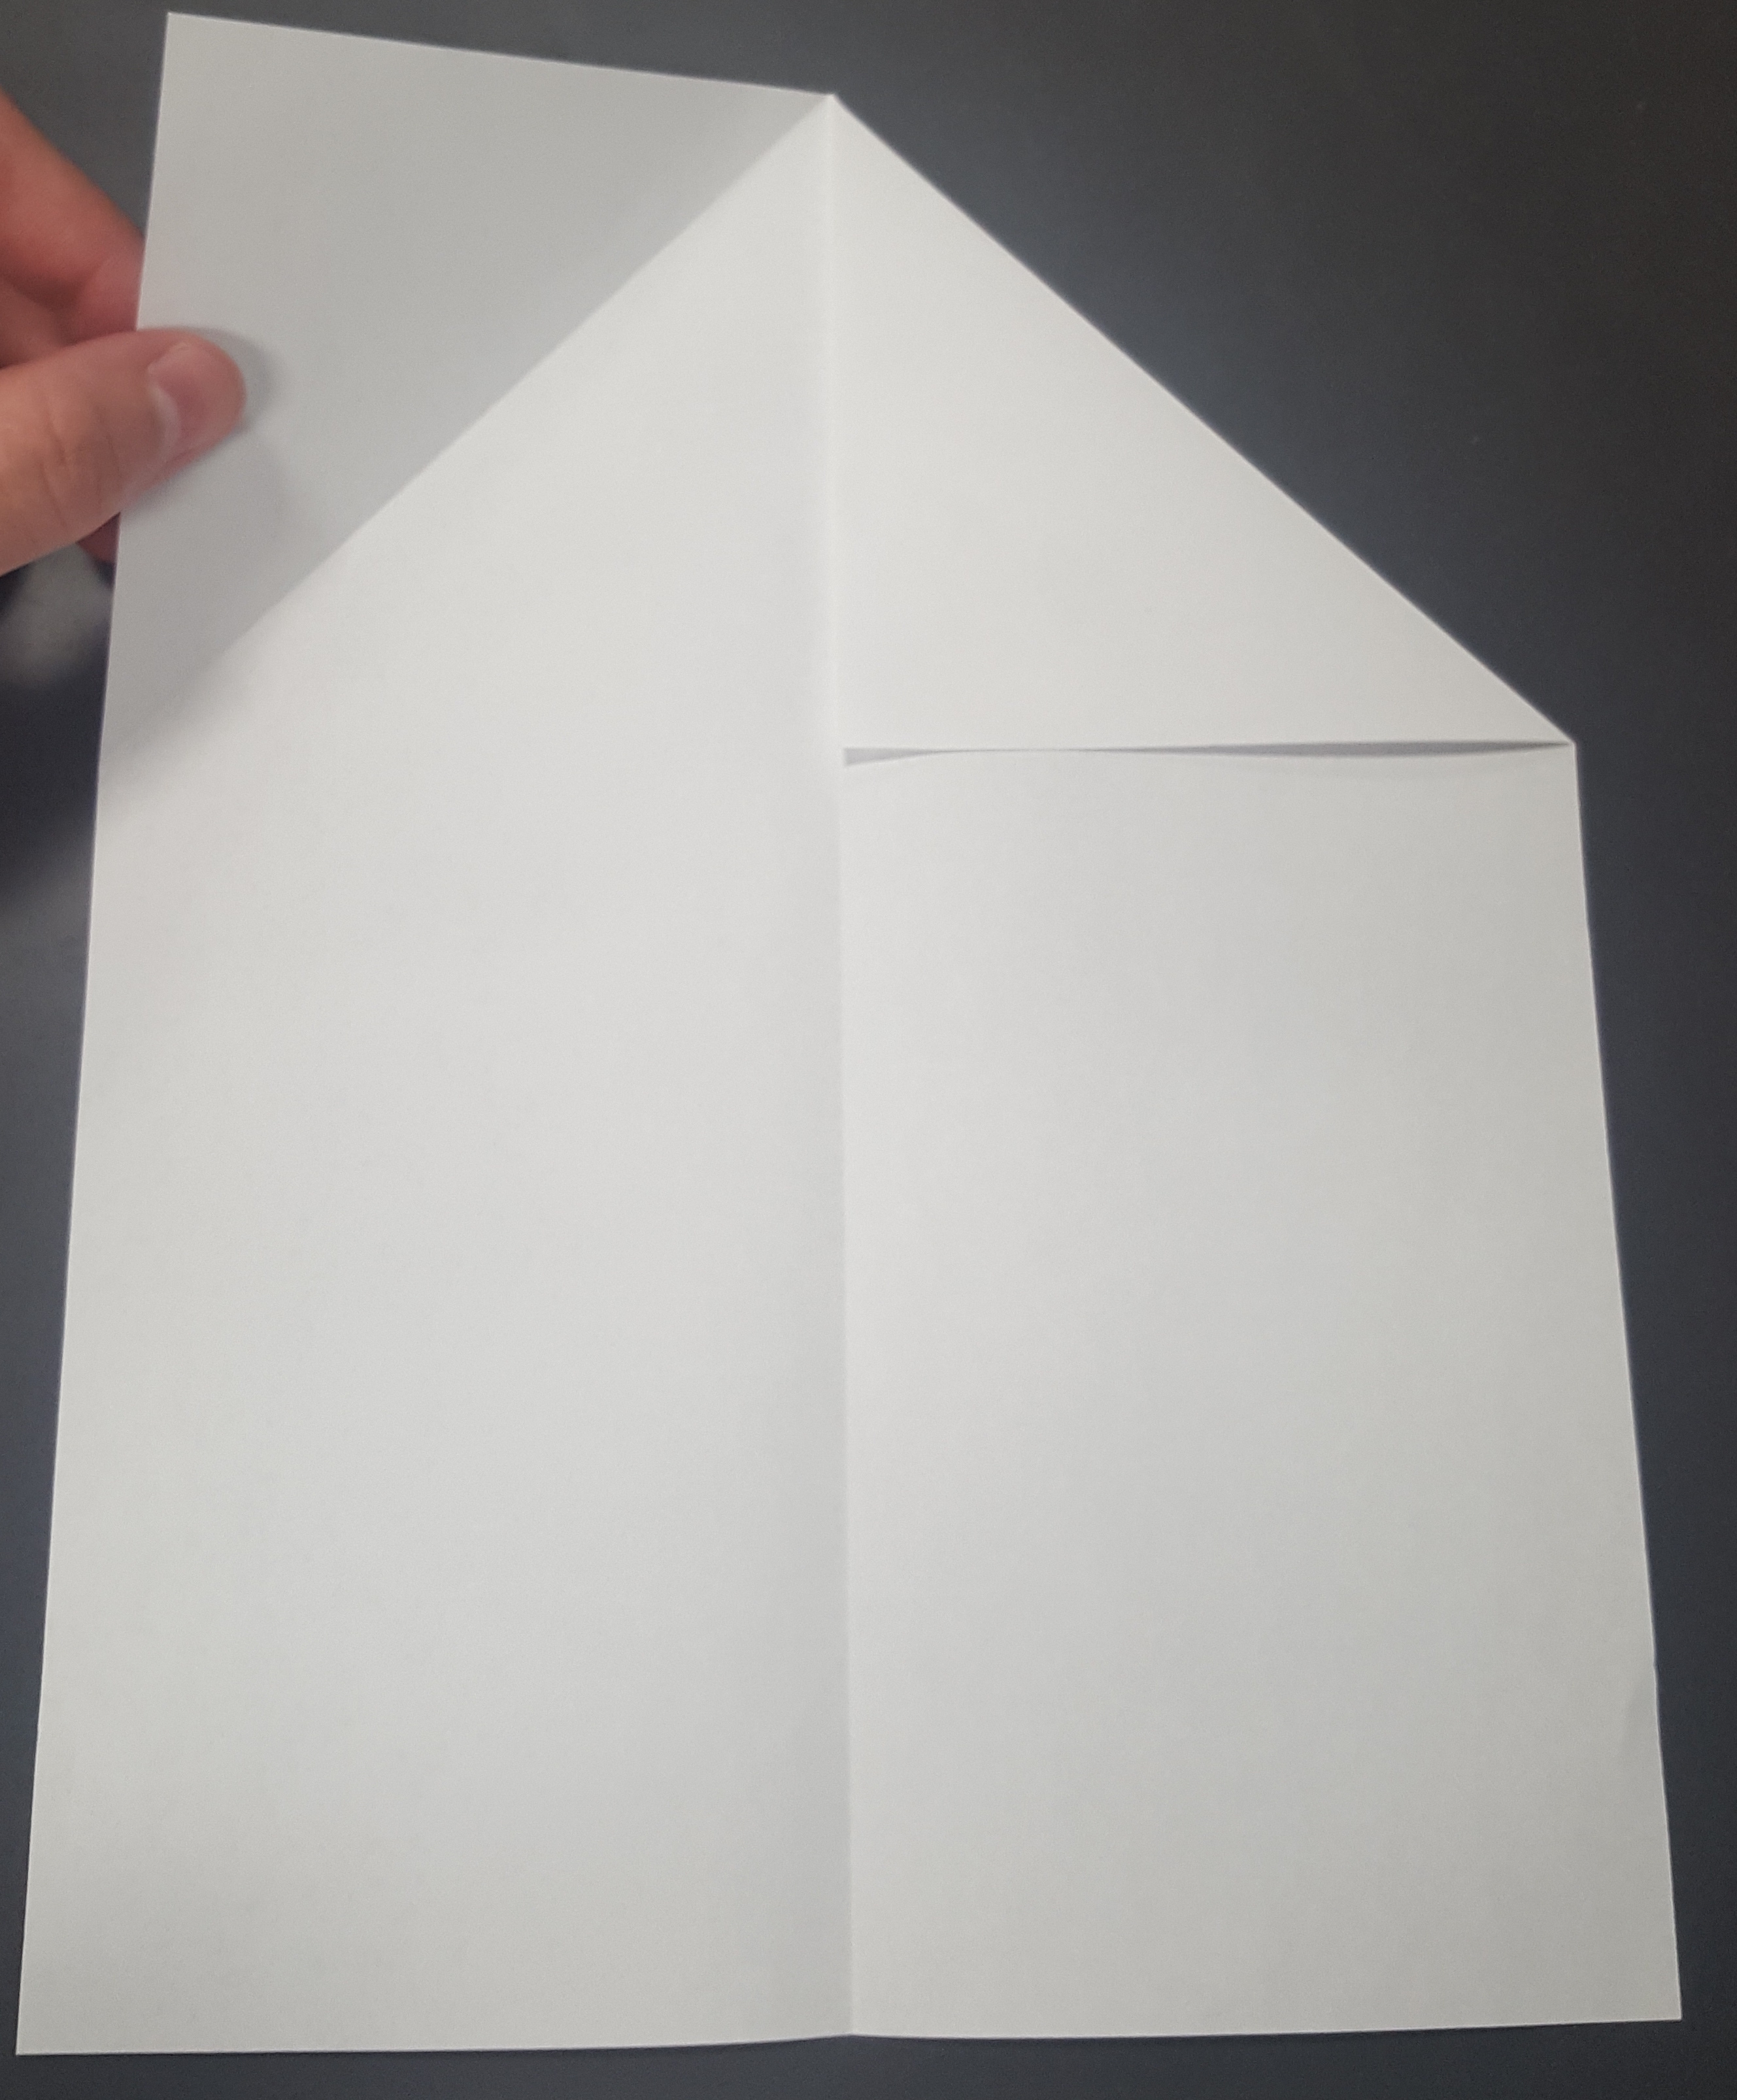
\includegraphics[width=.4\textwidth]{engl314/instructional/images/fourth.jpg} }}
\end{figure}

\begin{figure}[!h]
  \centering
  \caption{Flip the paper over and fold the corners in so they meet on the center crease.}
  \subfloat{{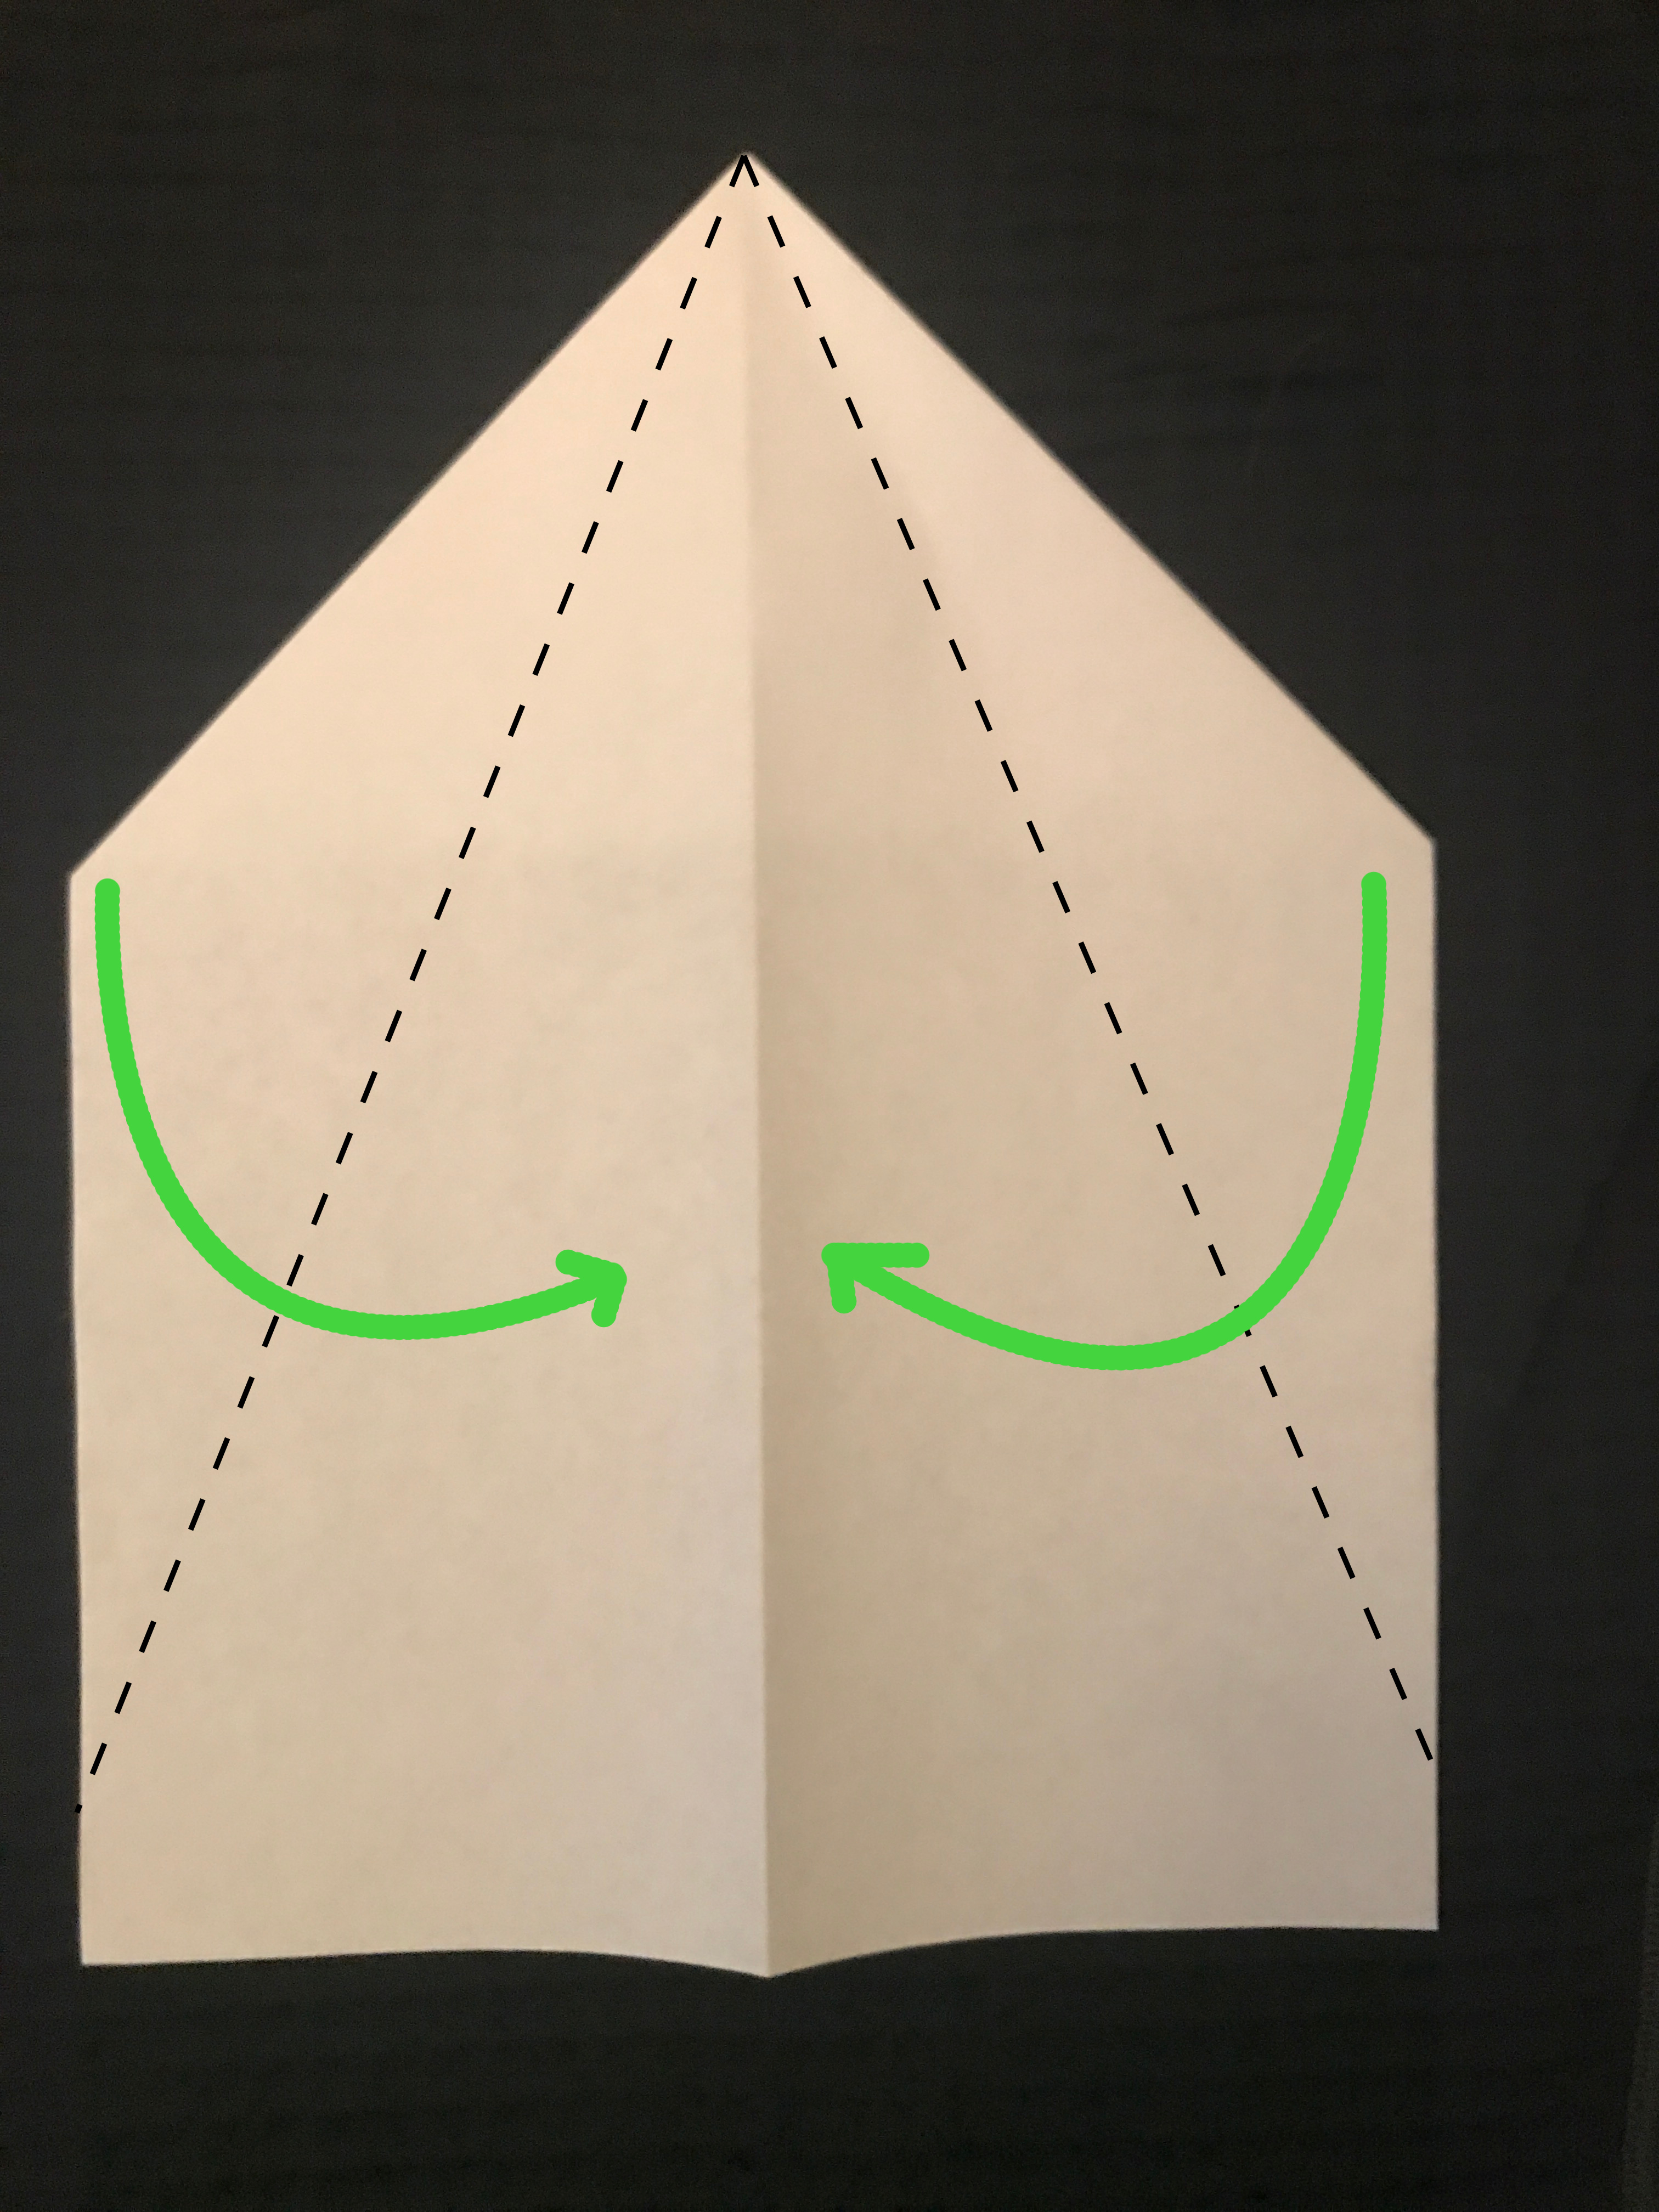
\includegraphics[width=0.4\textwidth]{engl314/instructional/images/fifth.jpg} }}
  \qquad
  \subfloat{{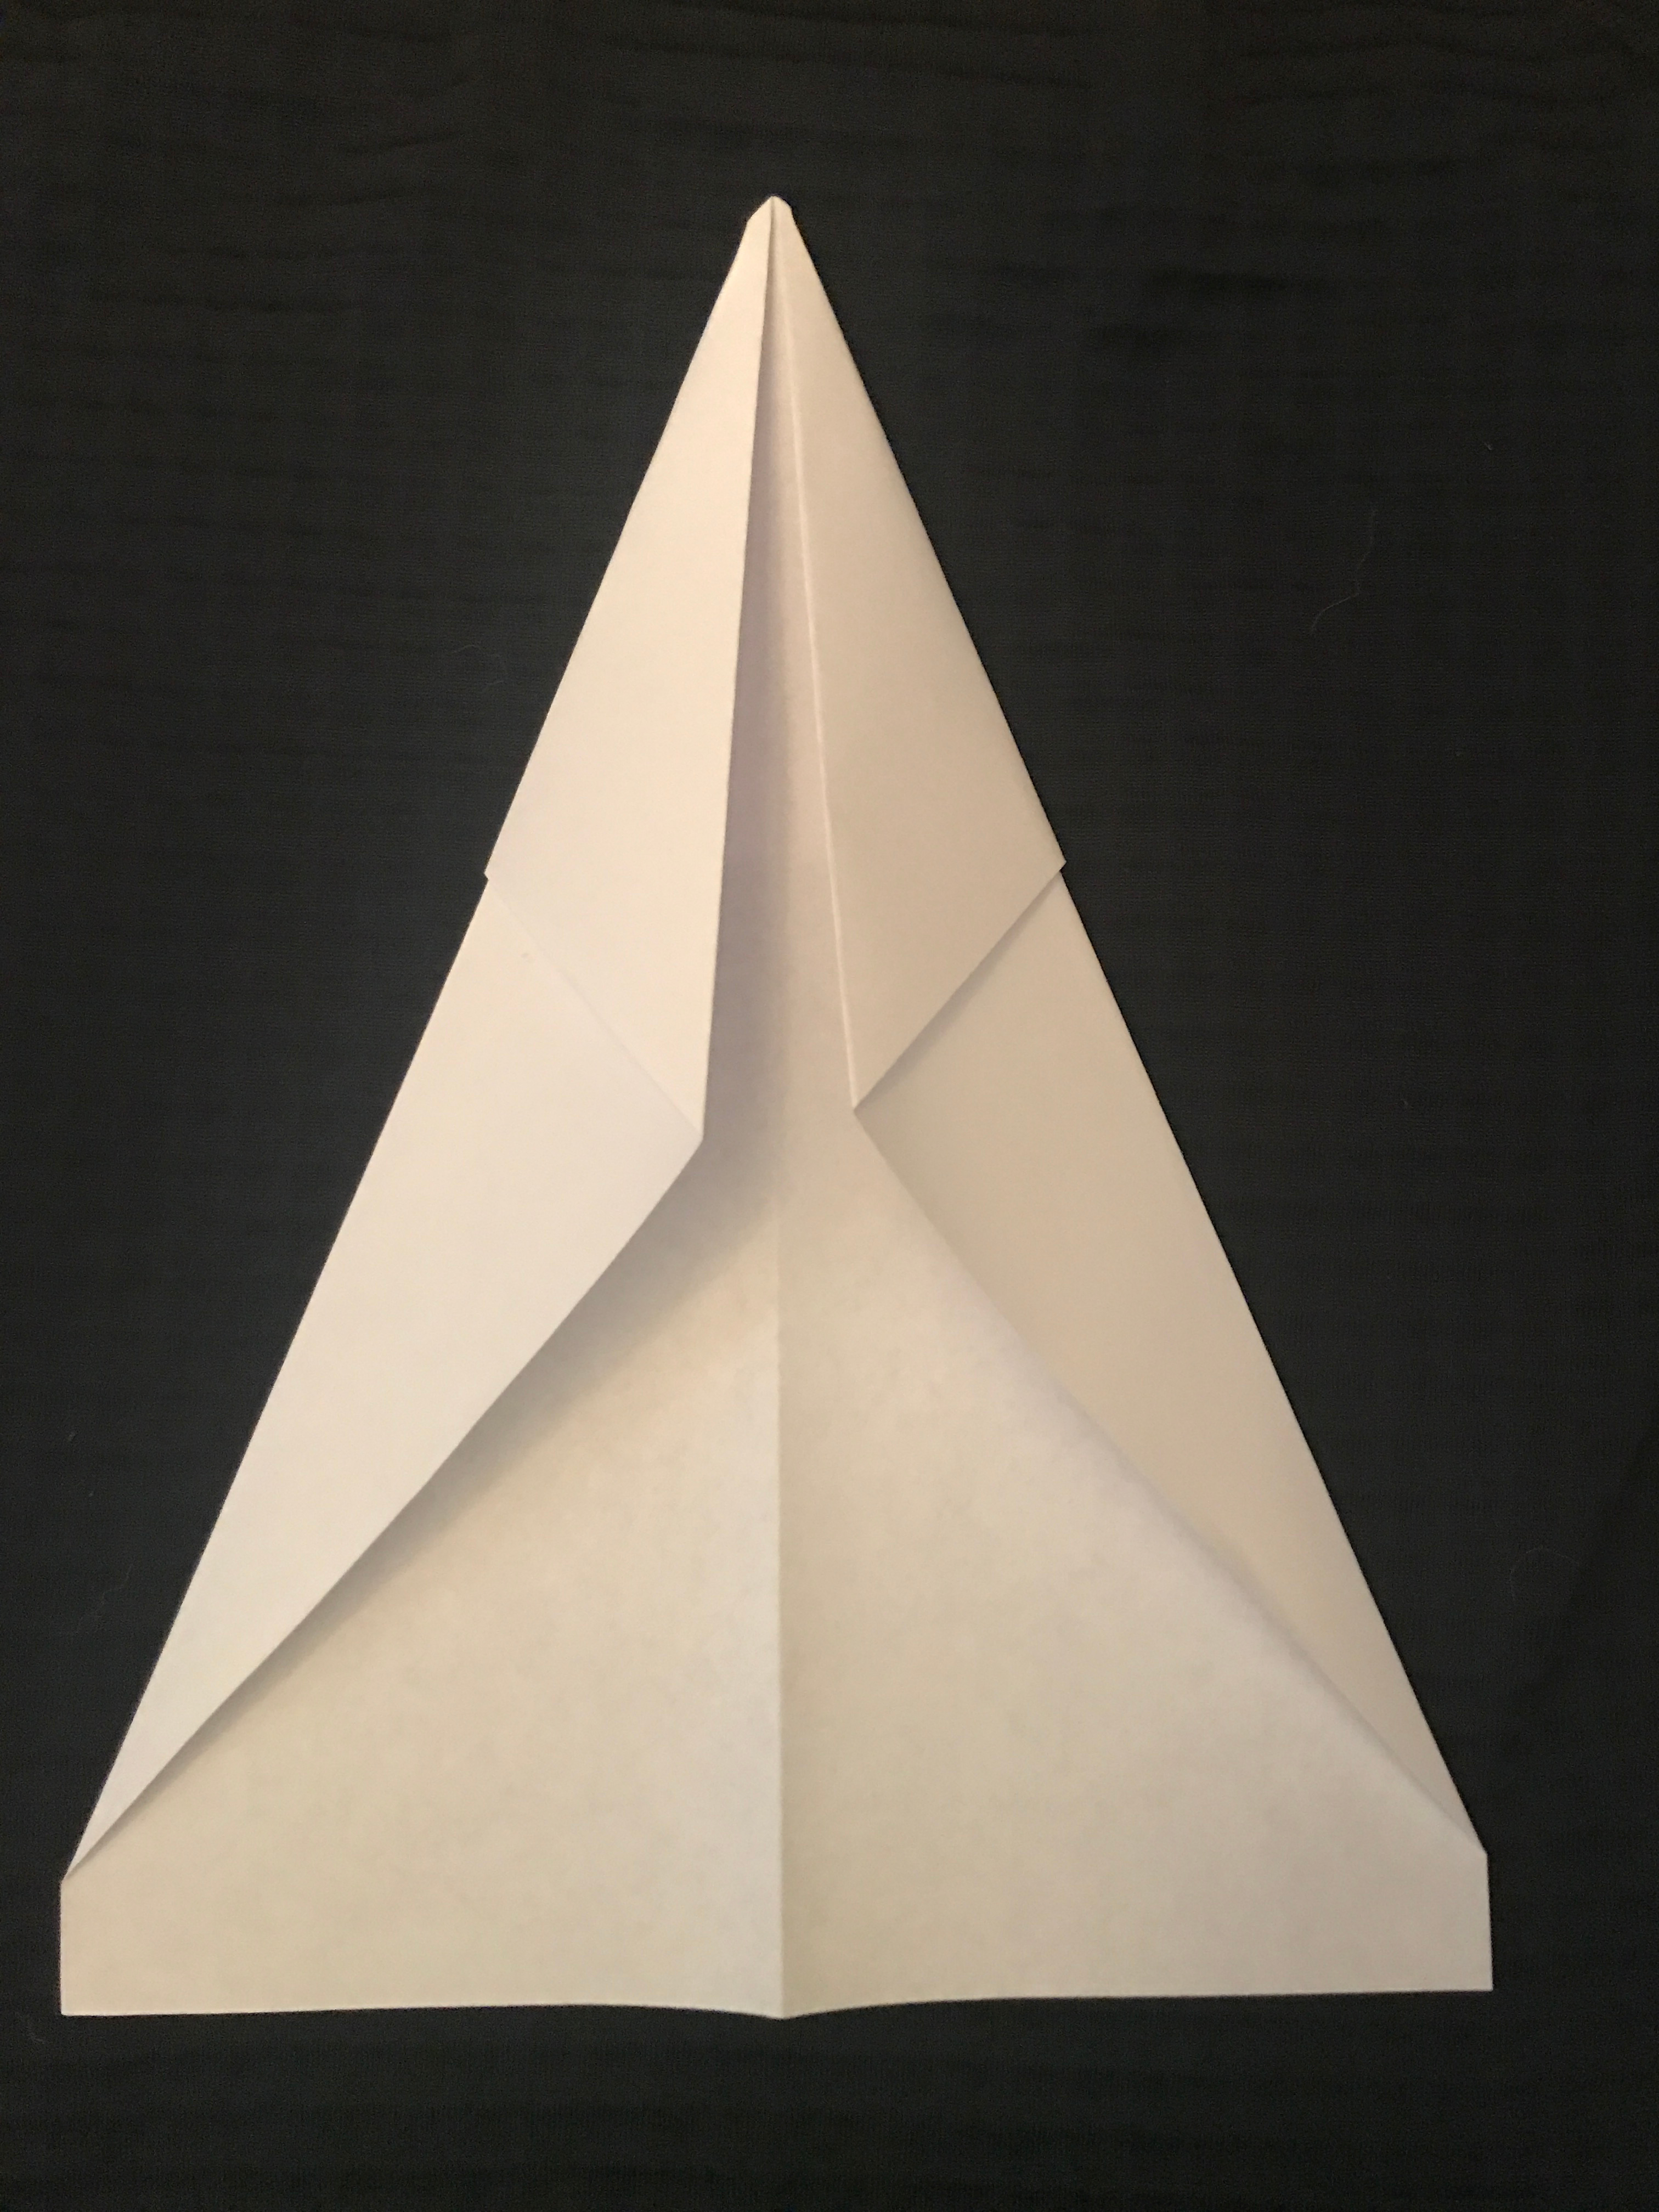
\includegraphics[width=.4\textwidth]{engl314/instructional/images/sixth.jpg} }}
\end{figure}
\clearpage

\begin{figure}[!t]
  \centering
  \caption{Fold the outside edges into the center so they they line up along the center fold.}
  \subfloat{{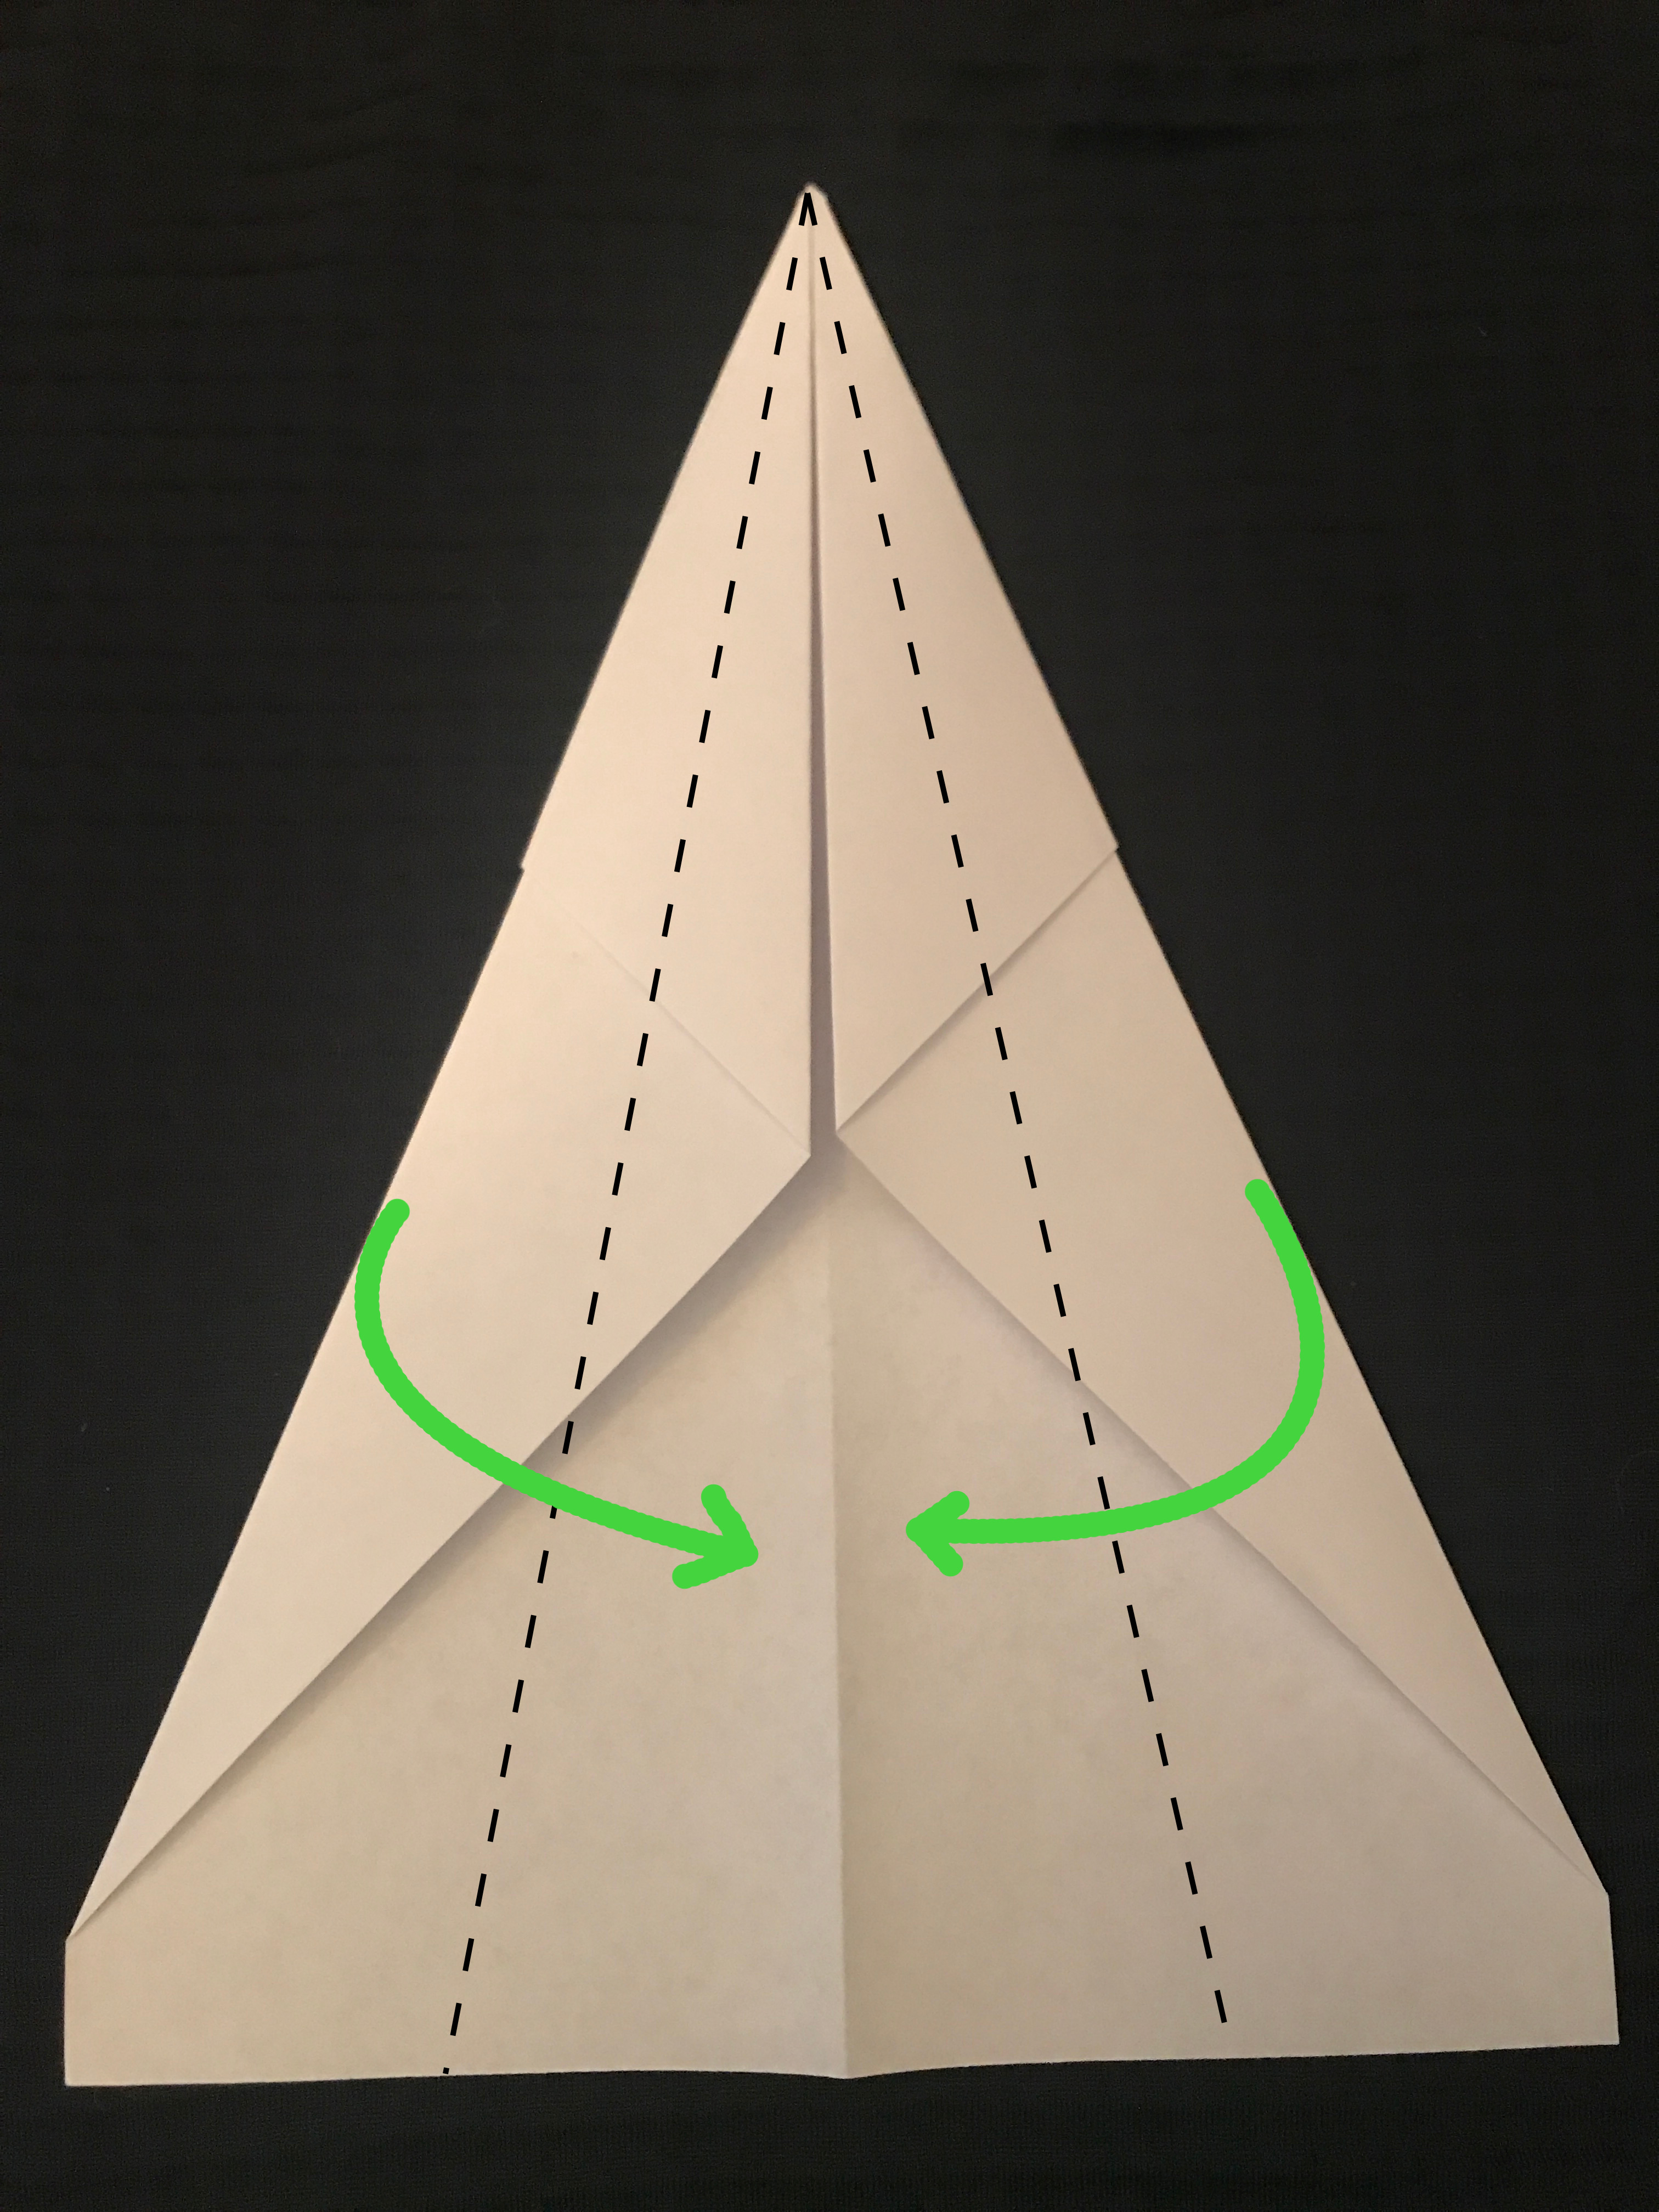
\includegraphics[width=0.4\textwidth]{engl314/instructional/images/seventh.jpg} }}
  \qquad
  \subfloat{{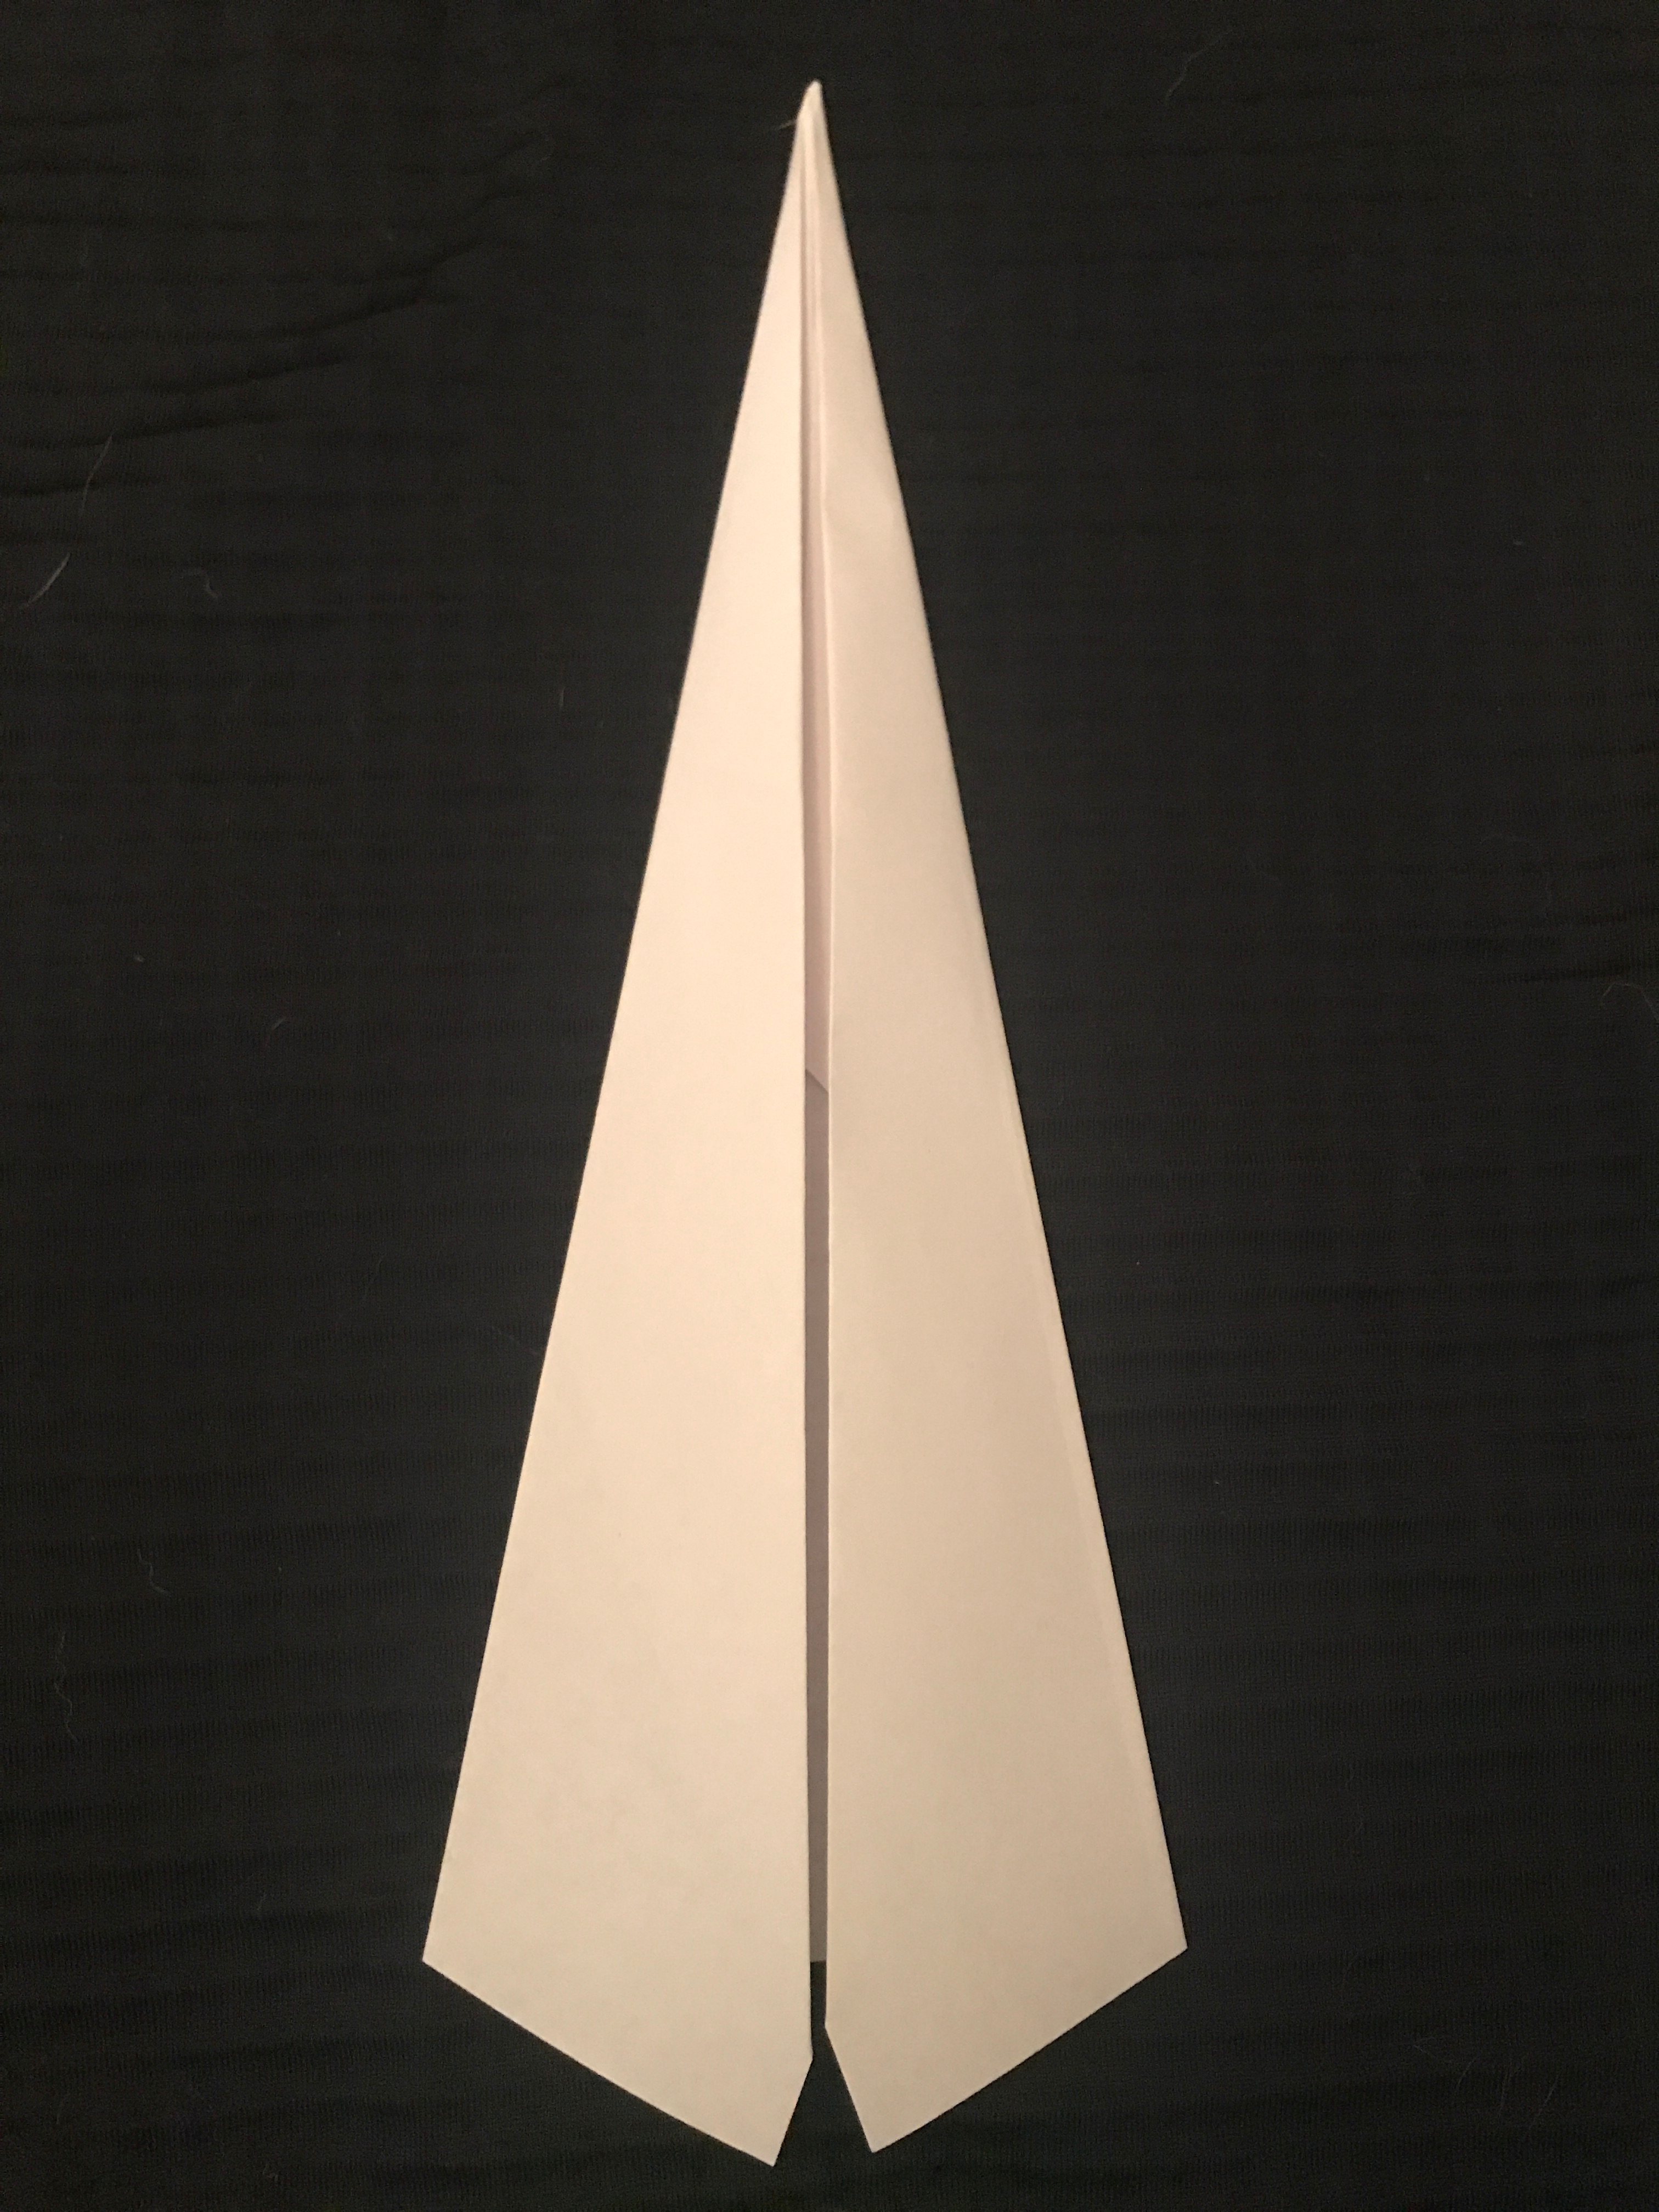
\includegraphics[width=.4\textwidth]{engl314/instructional/images/eight.jpg} }}
\end{figure}

\begin{figure}[!h]
  \centering
  \caption{Now unfold the last fold.}
  \subfloat{{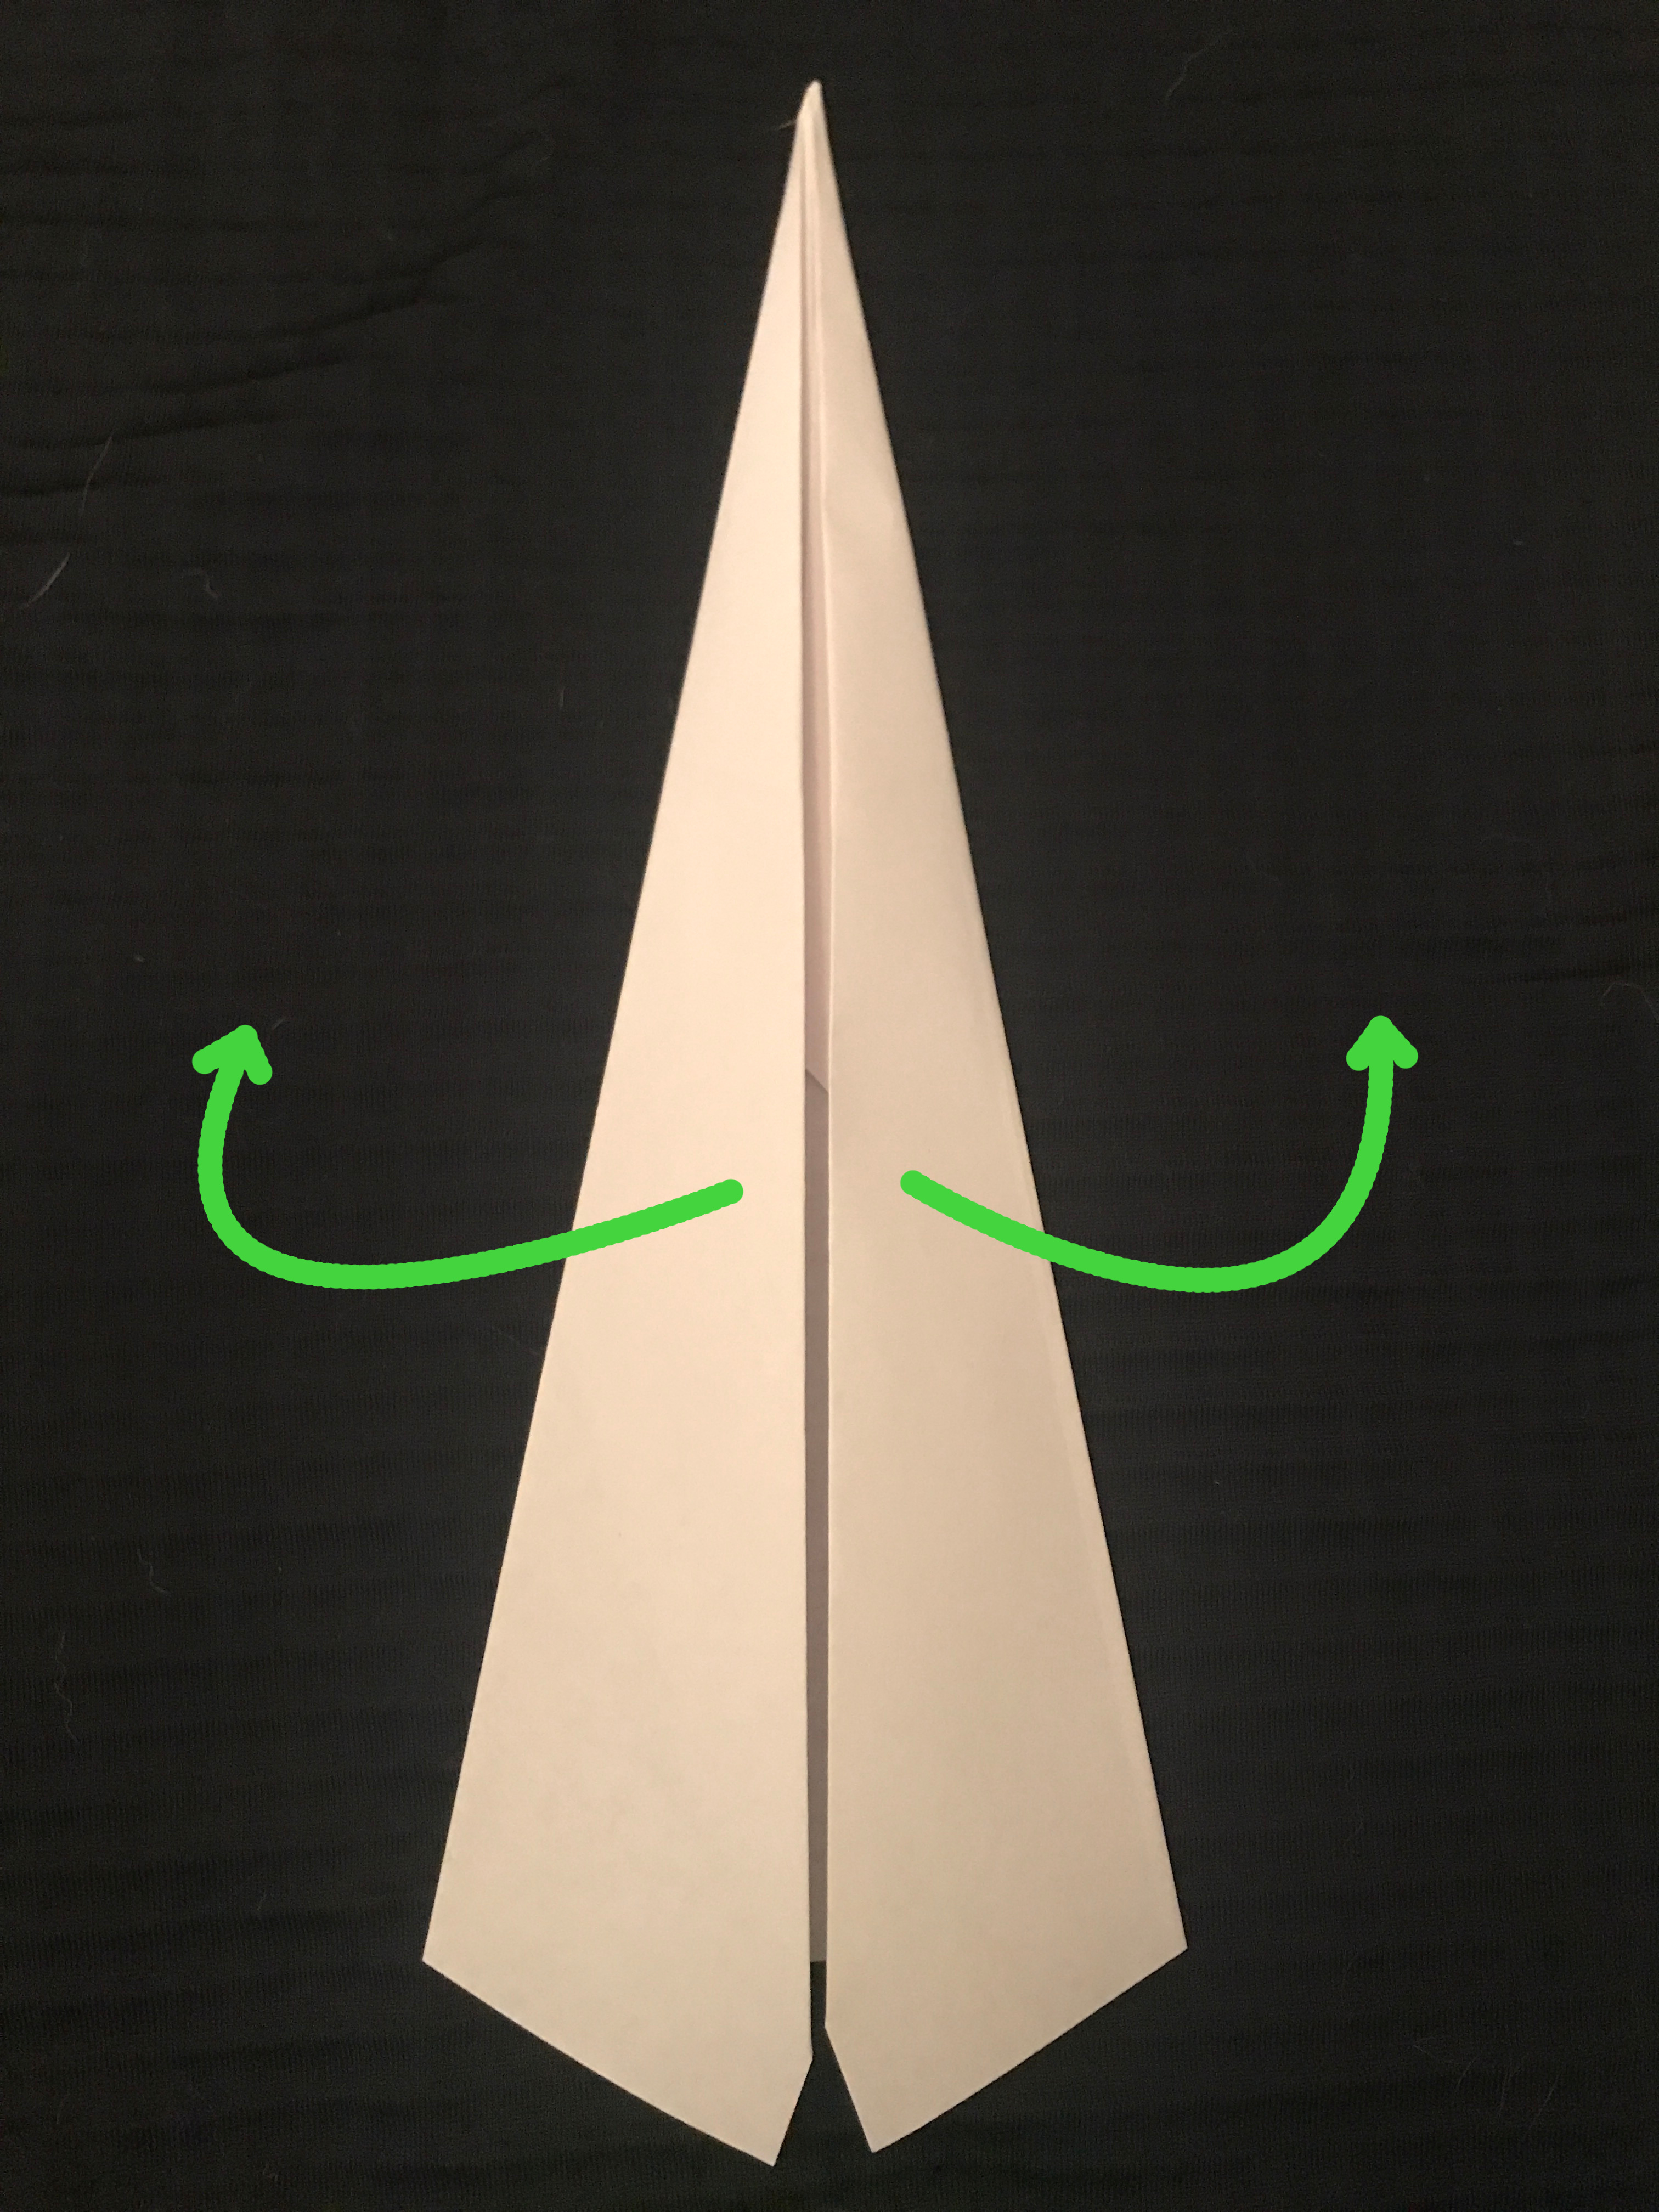
\includegraphics[width=0.4\textwidth]{engl314/instructional/images/nineth.jpg} }}
  \qquad
  \subfloat{{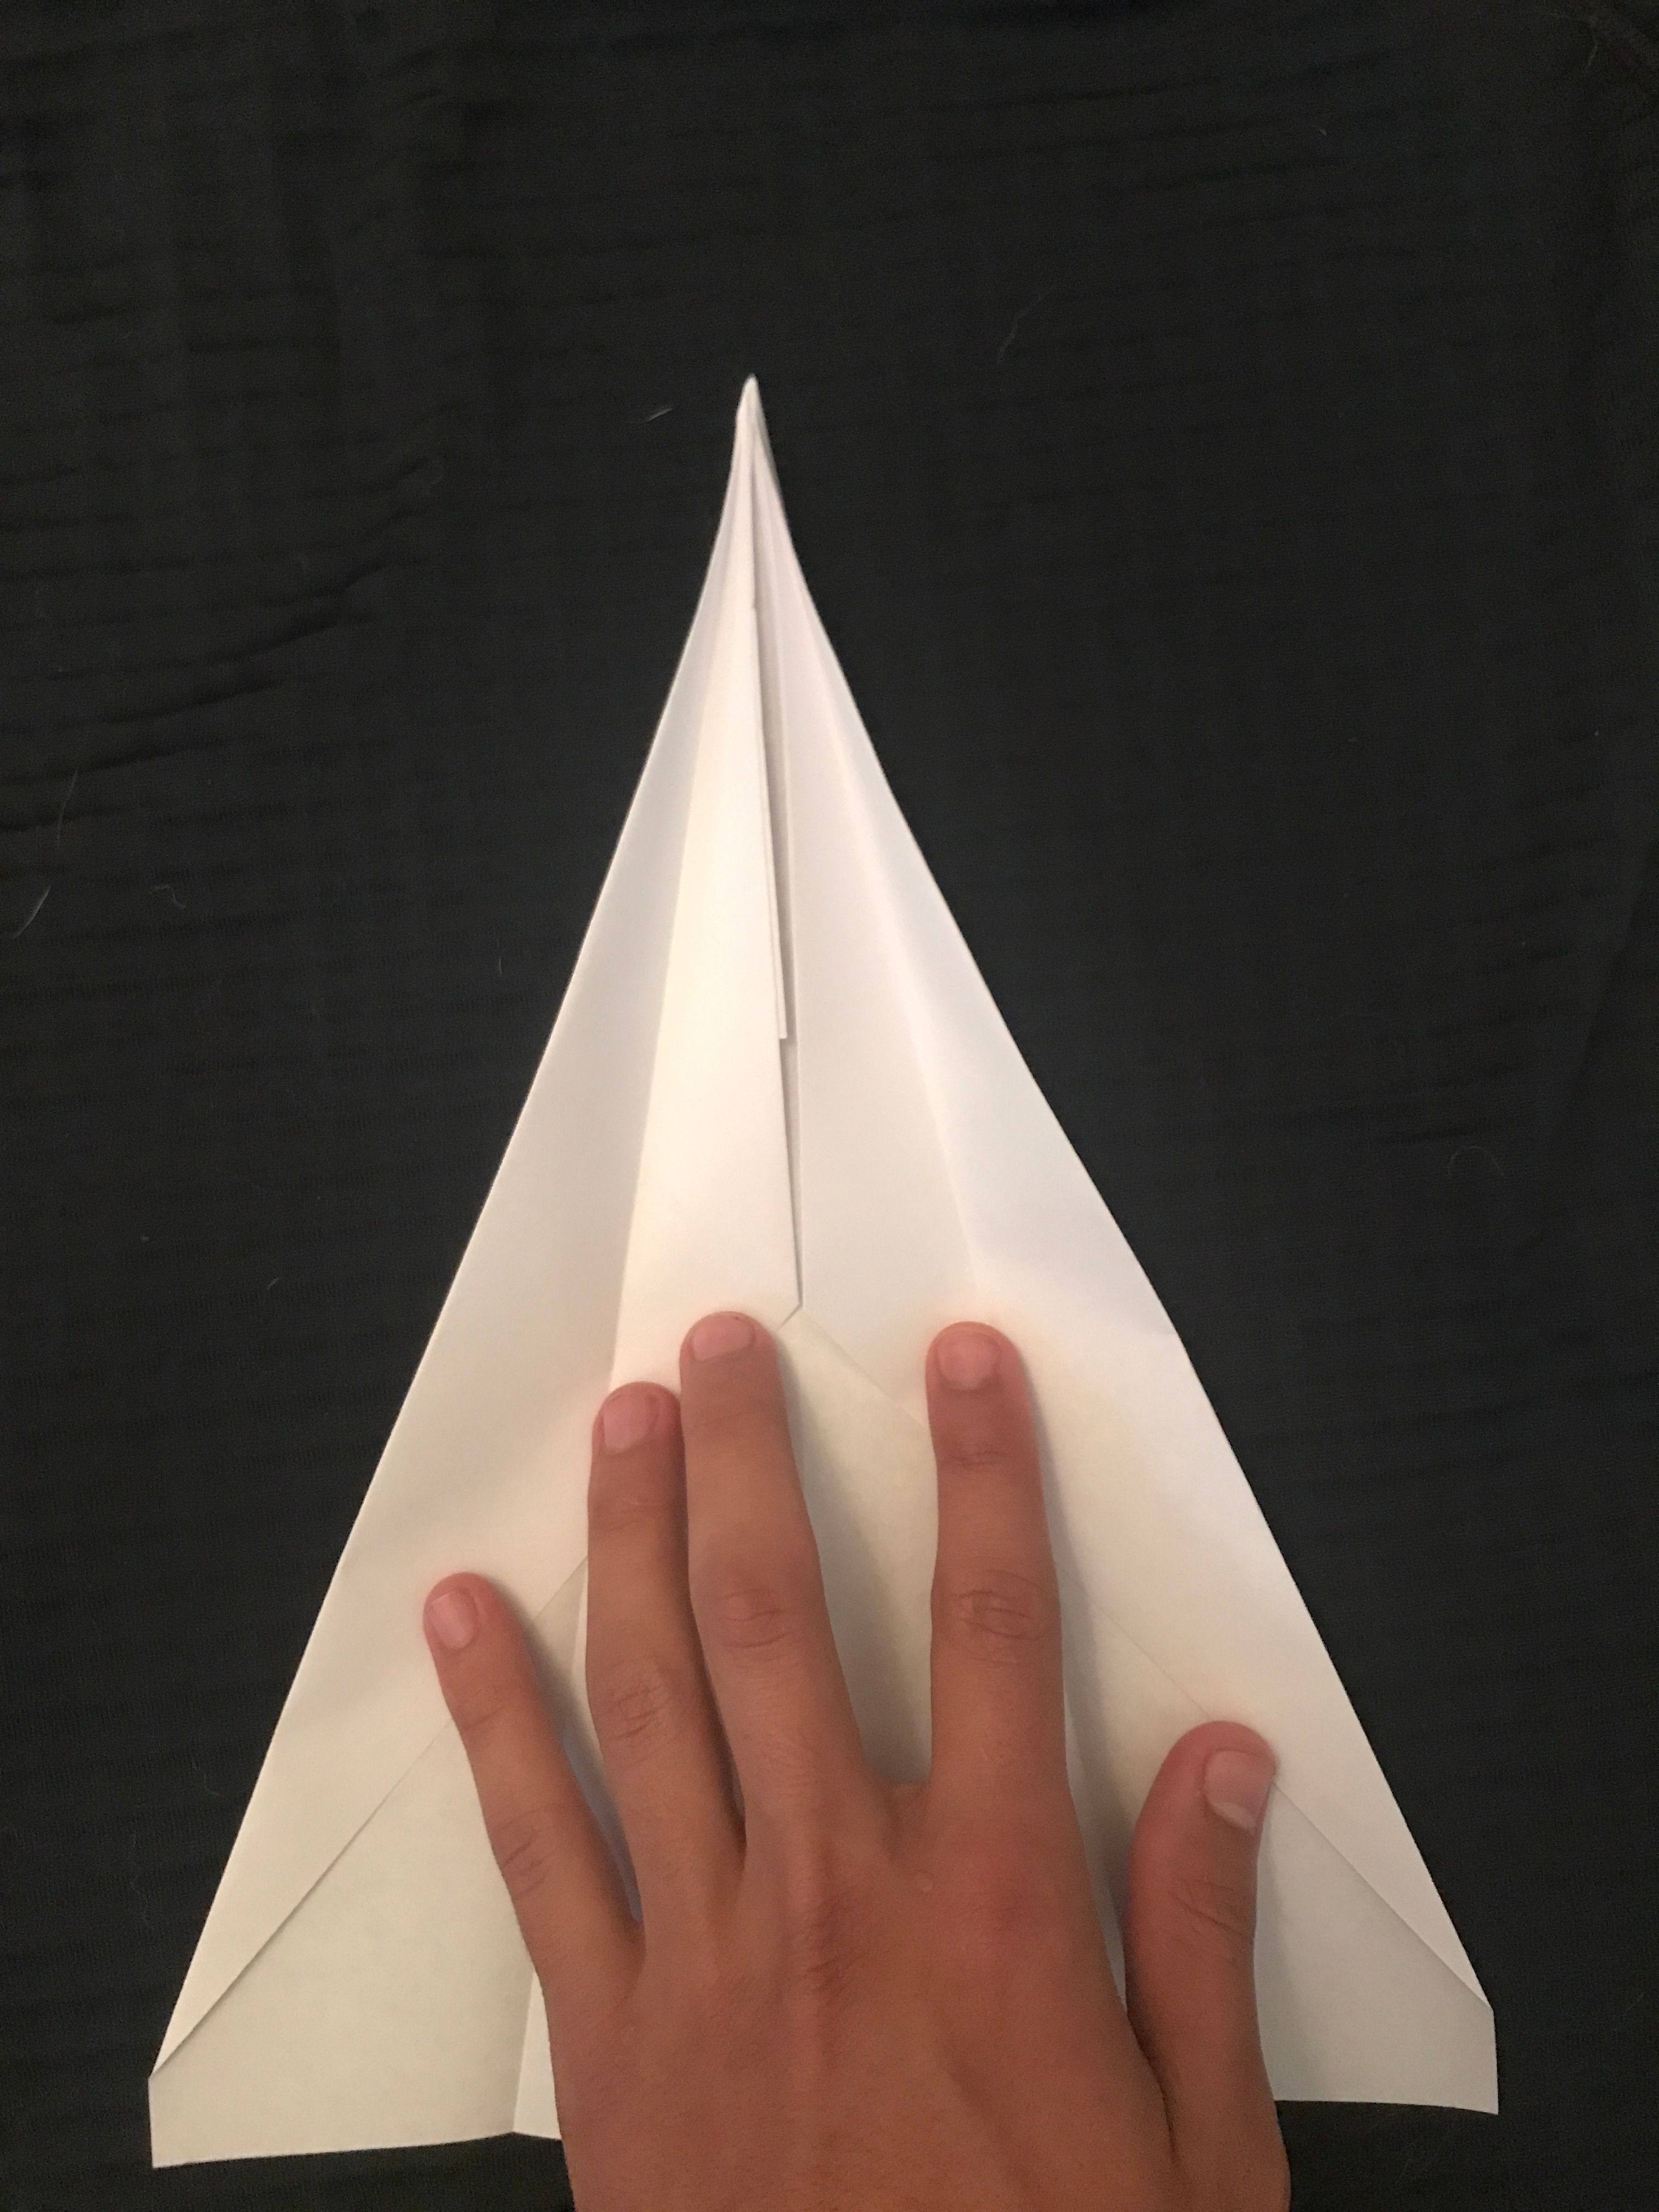
\includegraphics[width=.4\textwidth]{engl314/instructional/images/tenth.jpg} }}
\end{figure}

\begin{figure}[!t]
  \centering
  \caption{Pinch the center two sections together.}
  \subfloat{{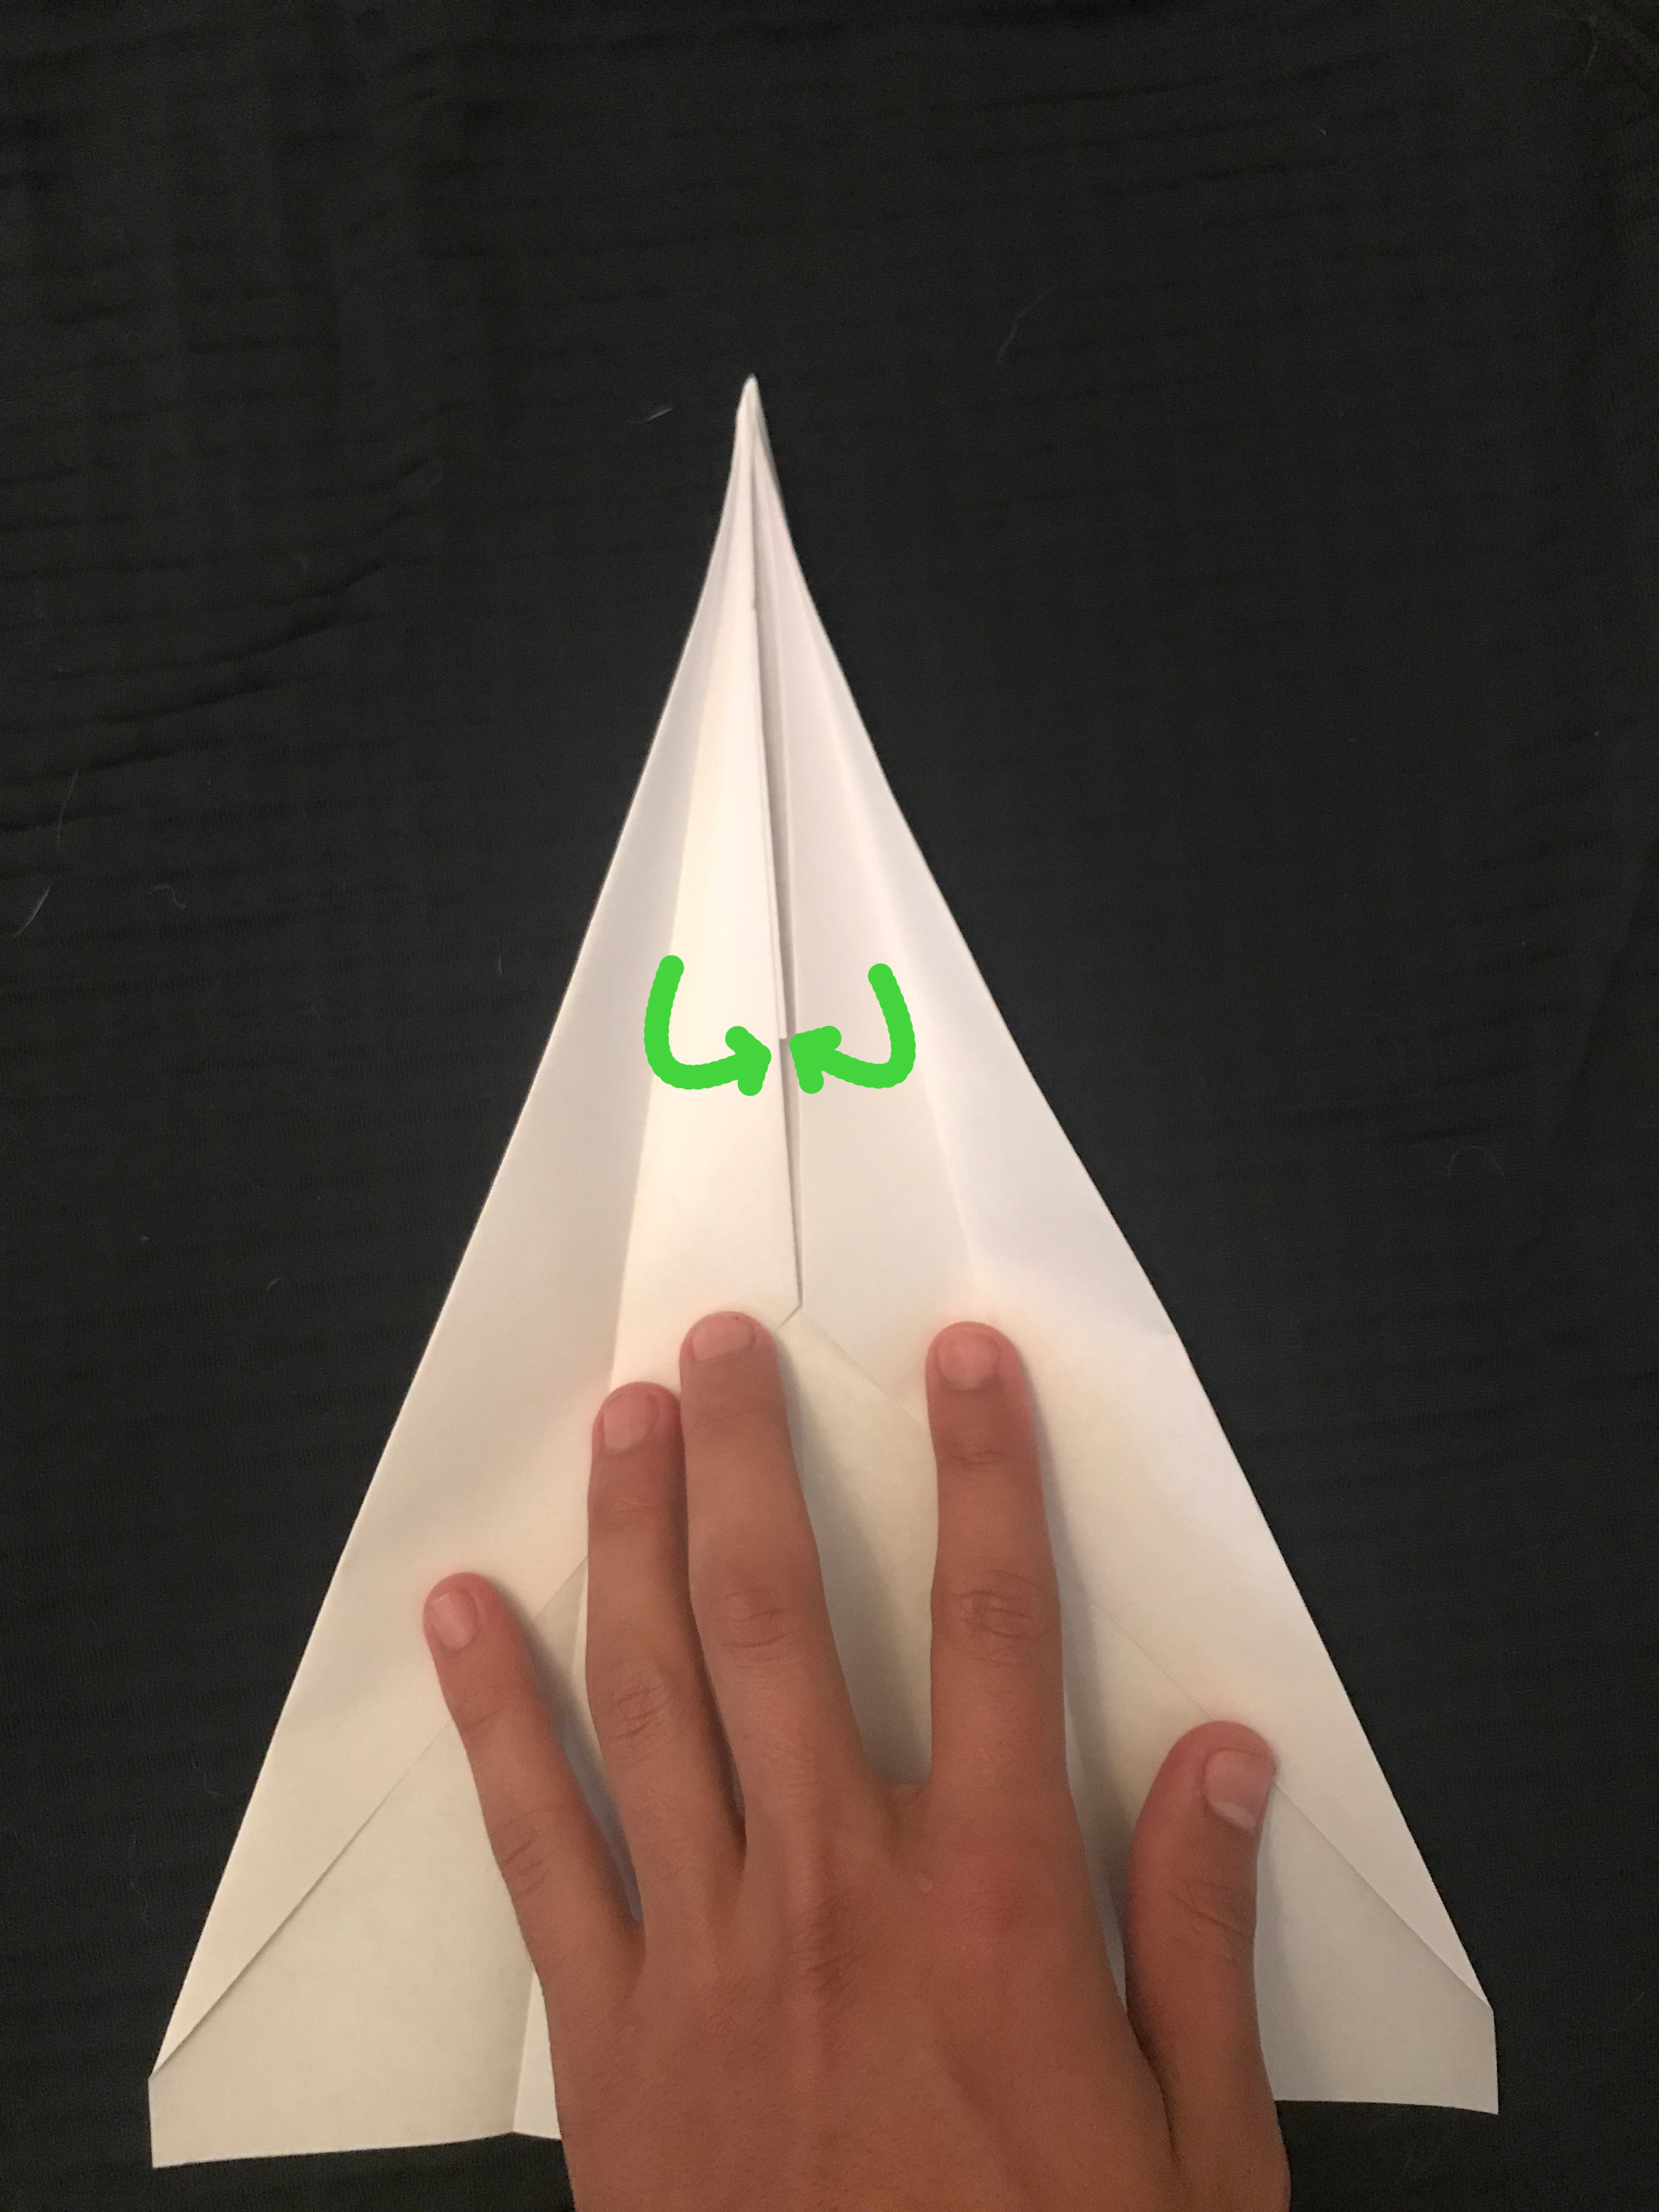
\includegraphics[width=0.4\textwidth]{engl314/instructional/images/eleventh.jpg} }}
  \qquad
  \subfloat{{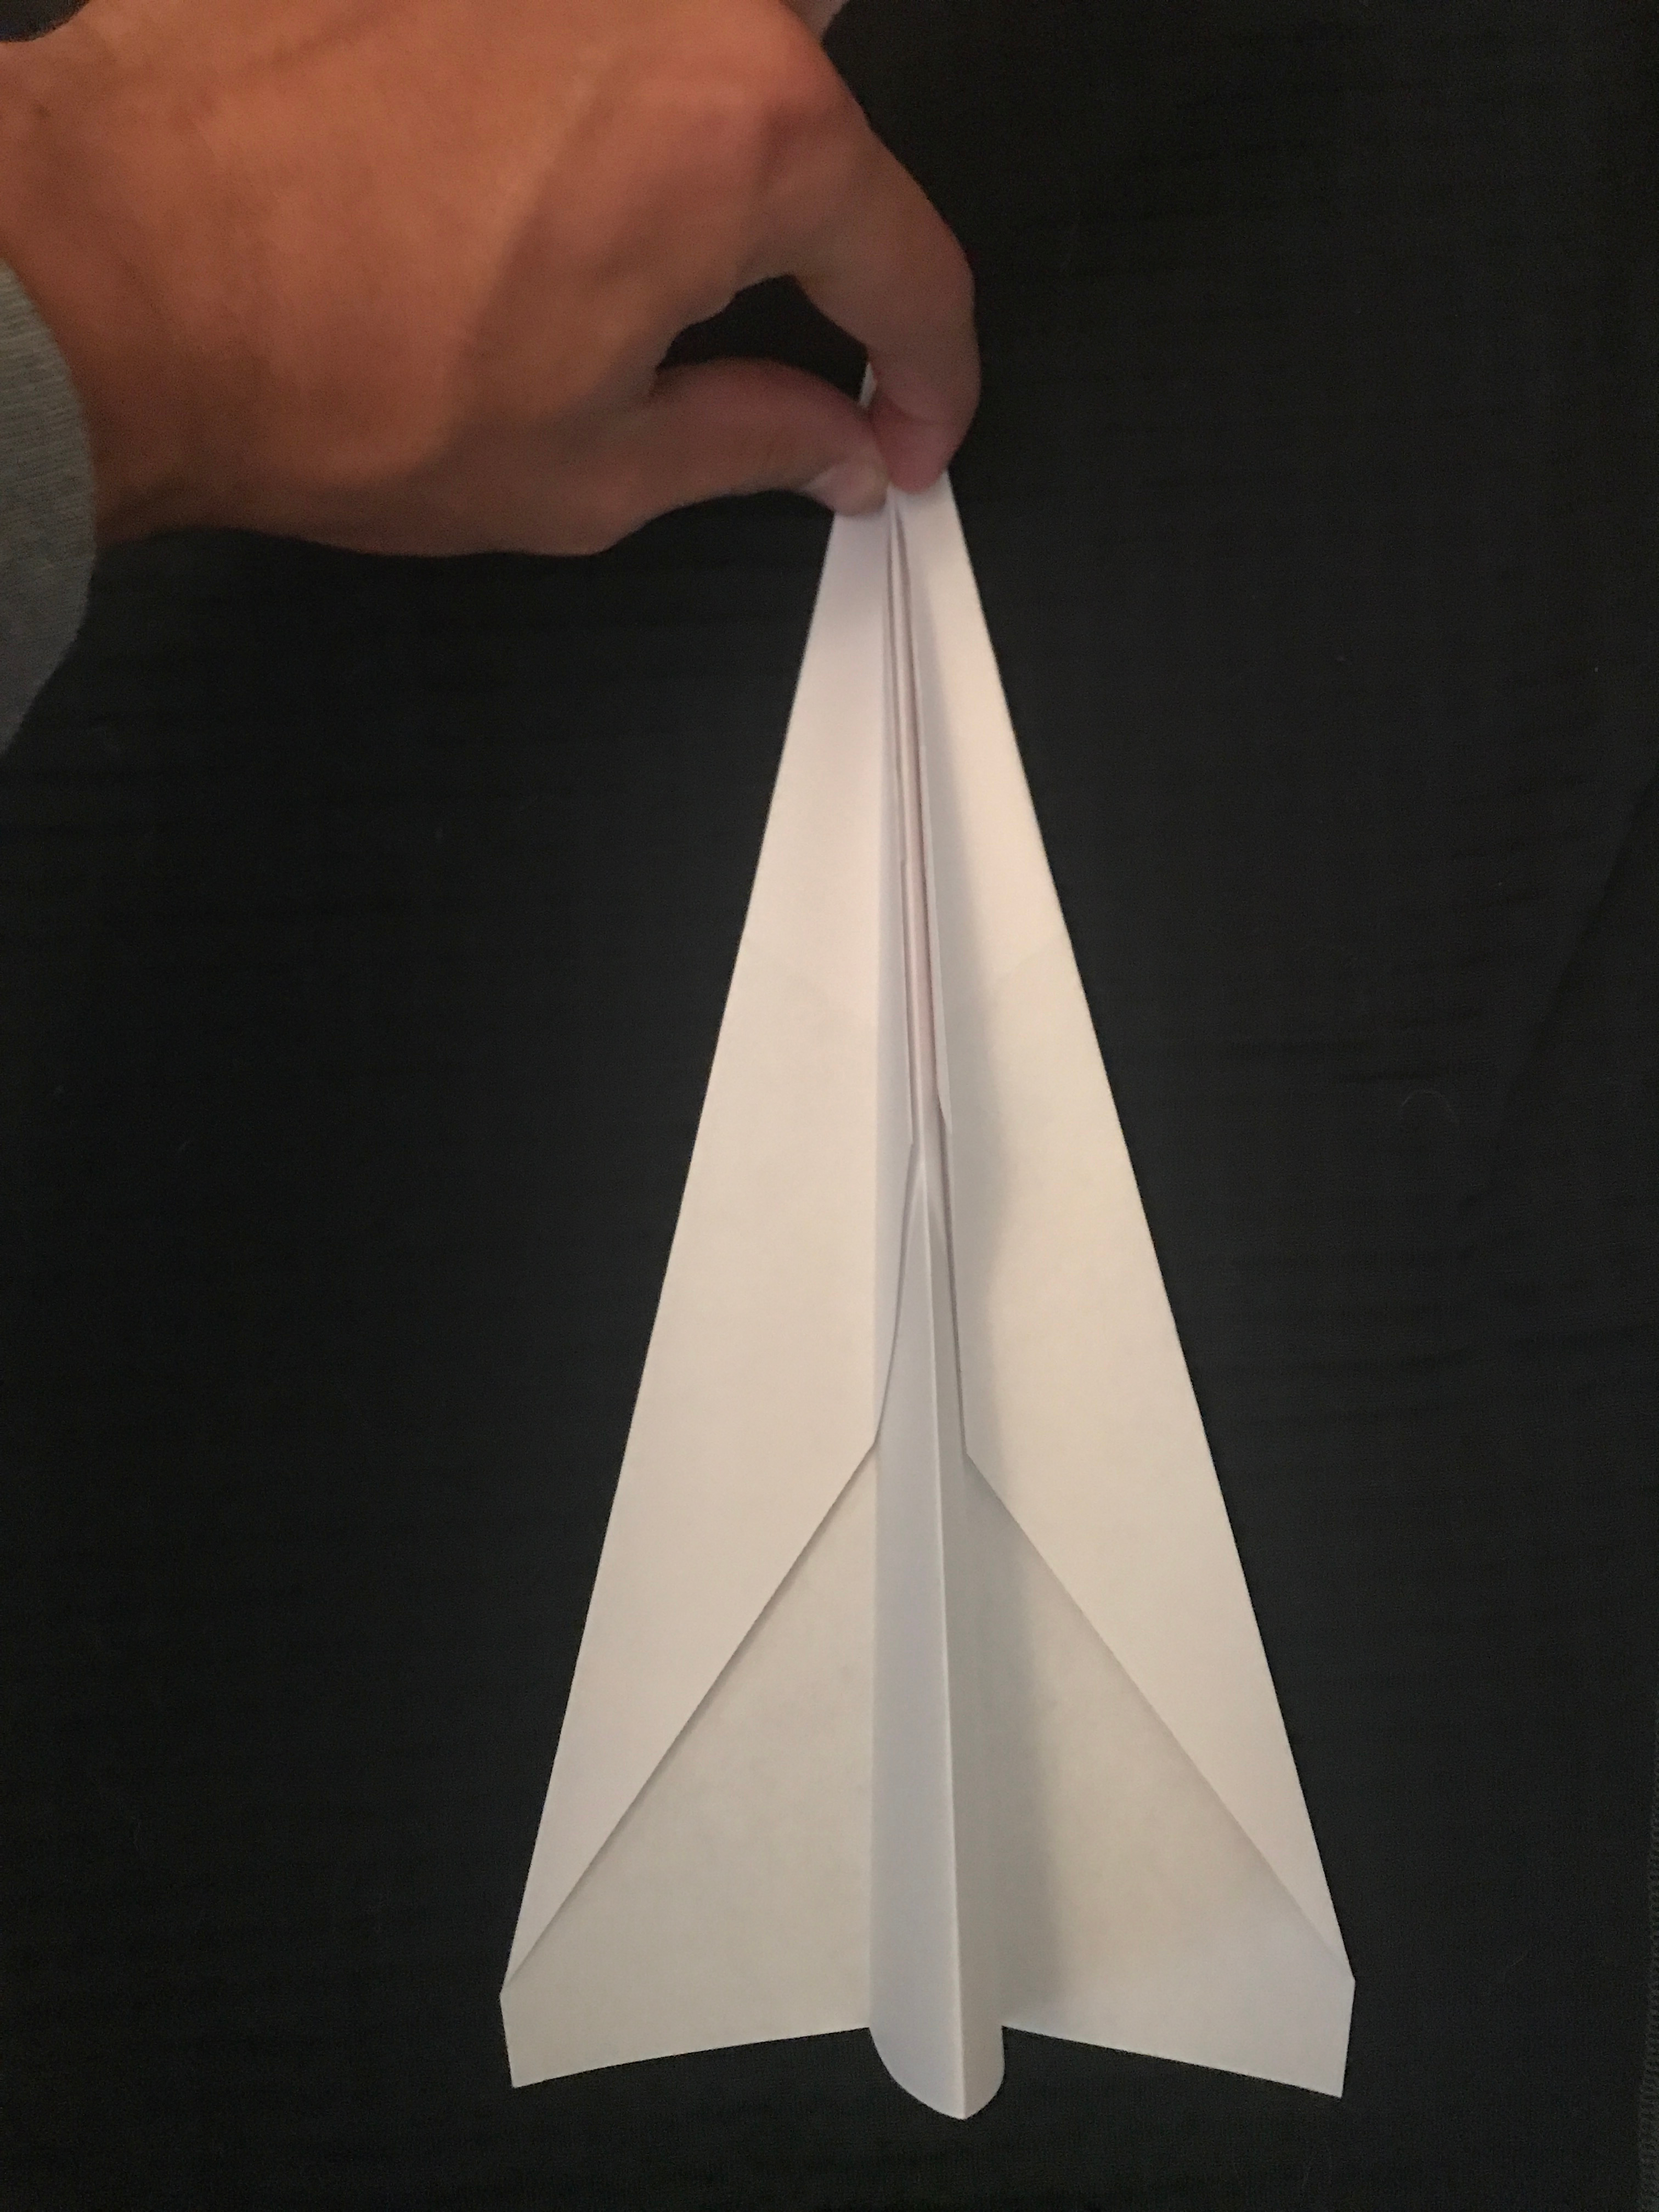
\includegraphics[width=.4\textwidth]{engl314/instructional/images/twelveth.jpg} }}
\end{figure}

\begin{figure}[!h]
  \centering
  \caption{You now have a paper airplane. optionally you can draw flames on it to increase its speed.}
  \subfloat{{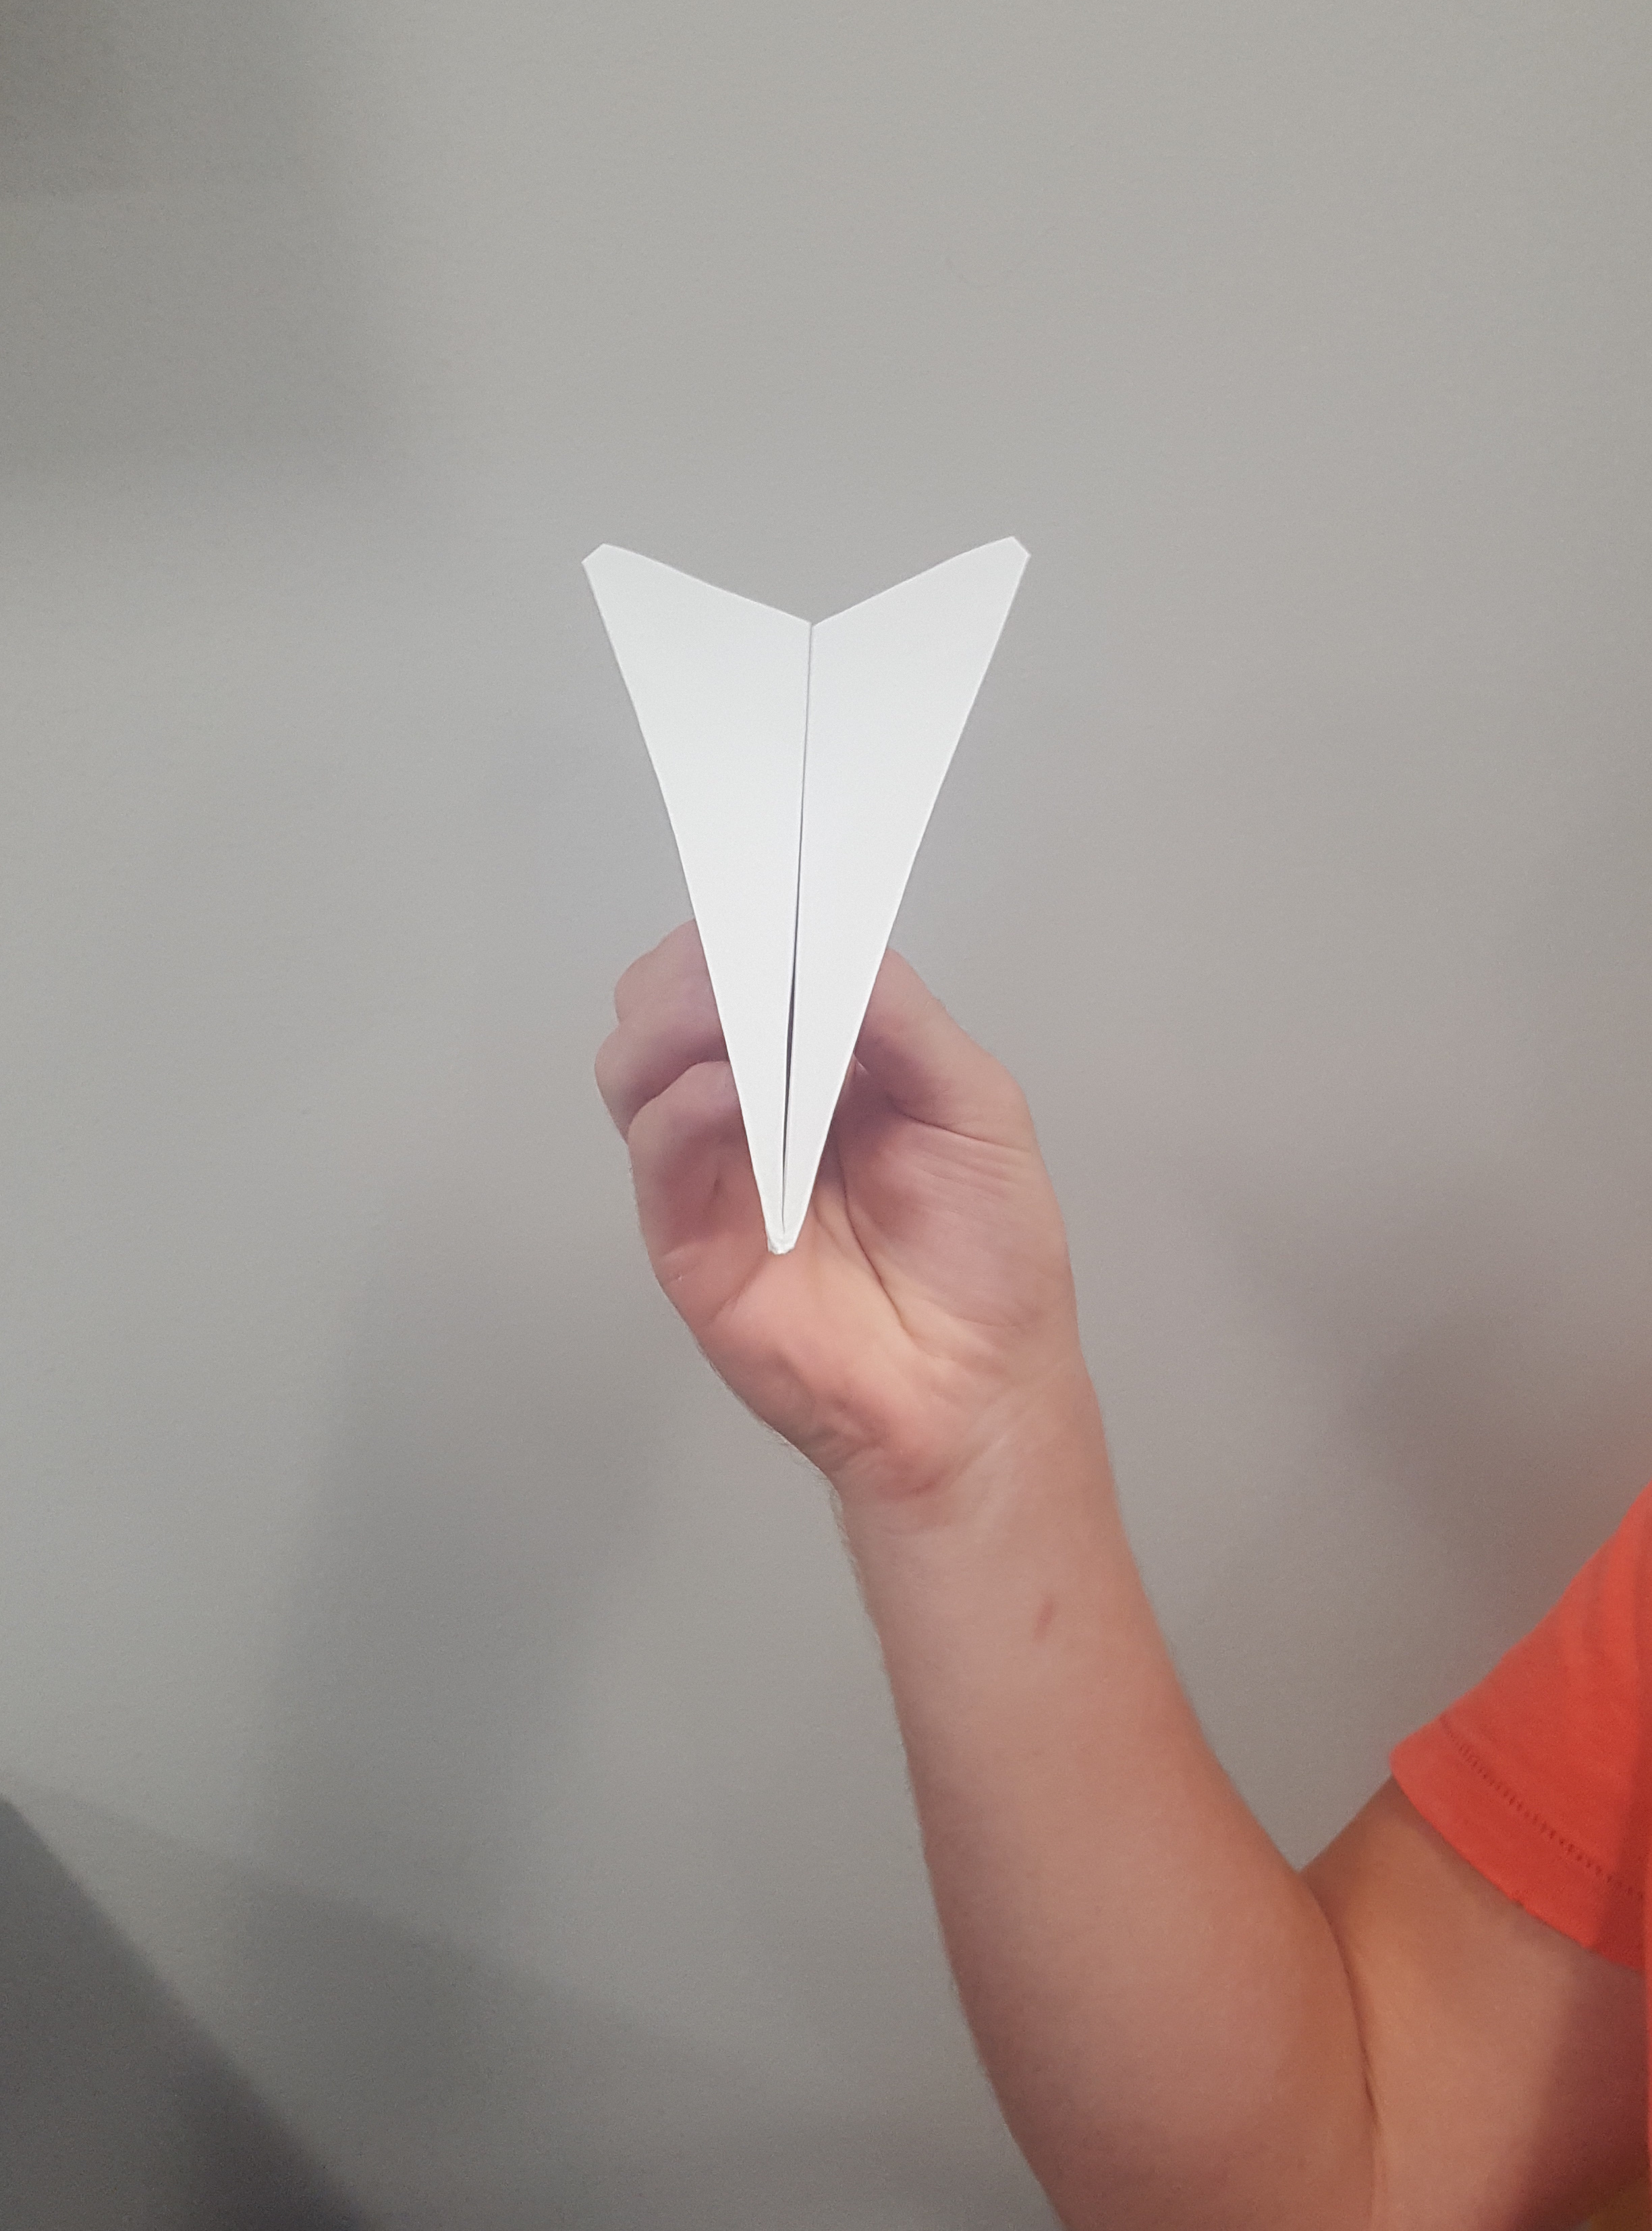
\includegraphics[width=0.4\textwidth]{engl314/instructional/images/thirteenth.jpg} }}
  \qquad
  \subfloat{{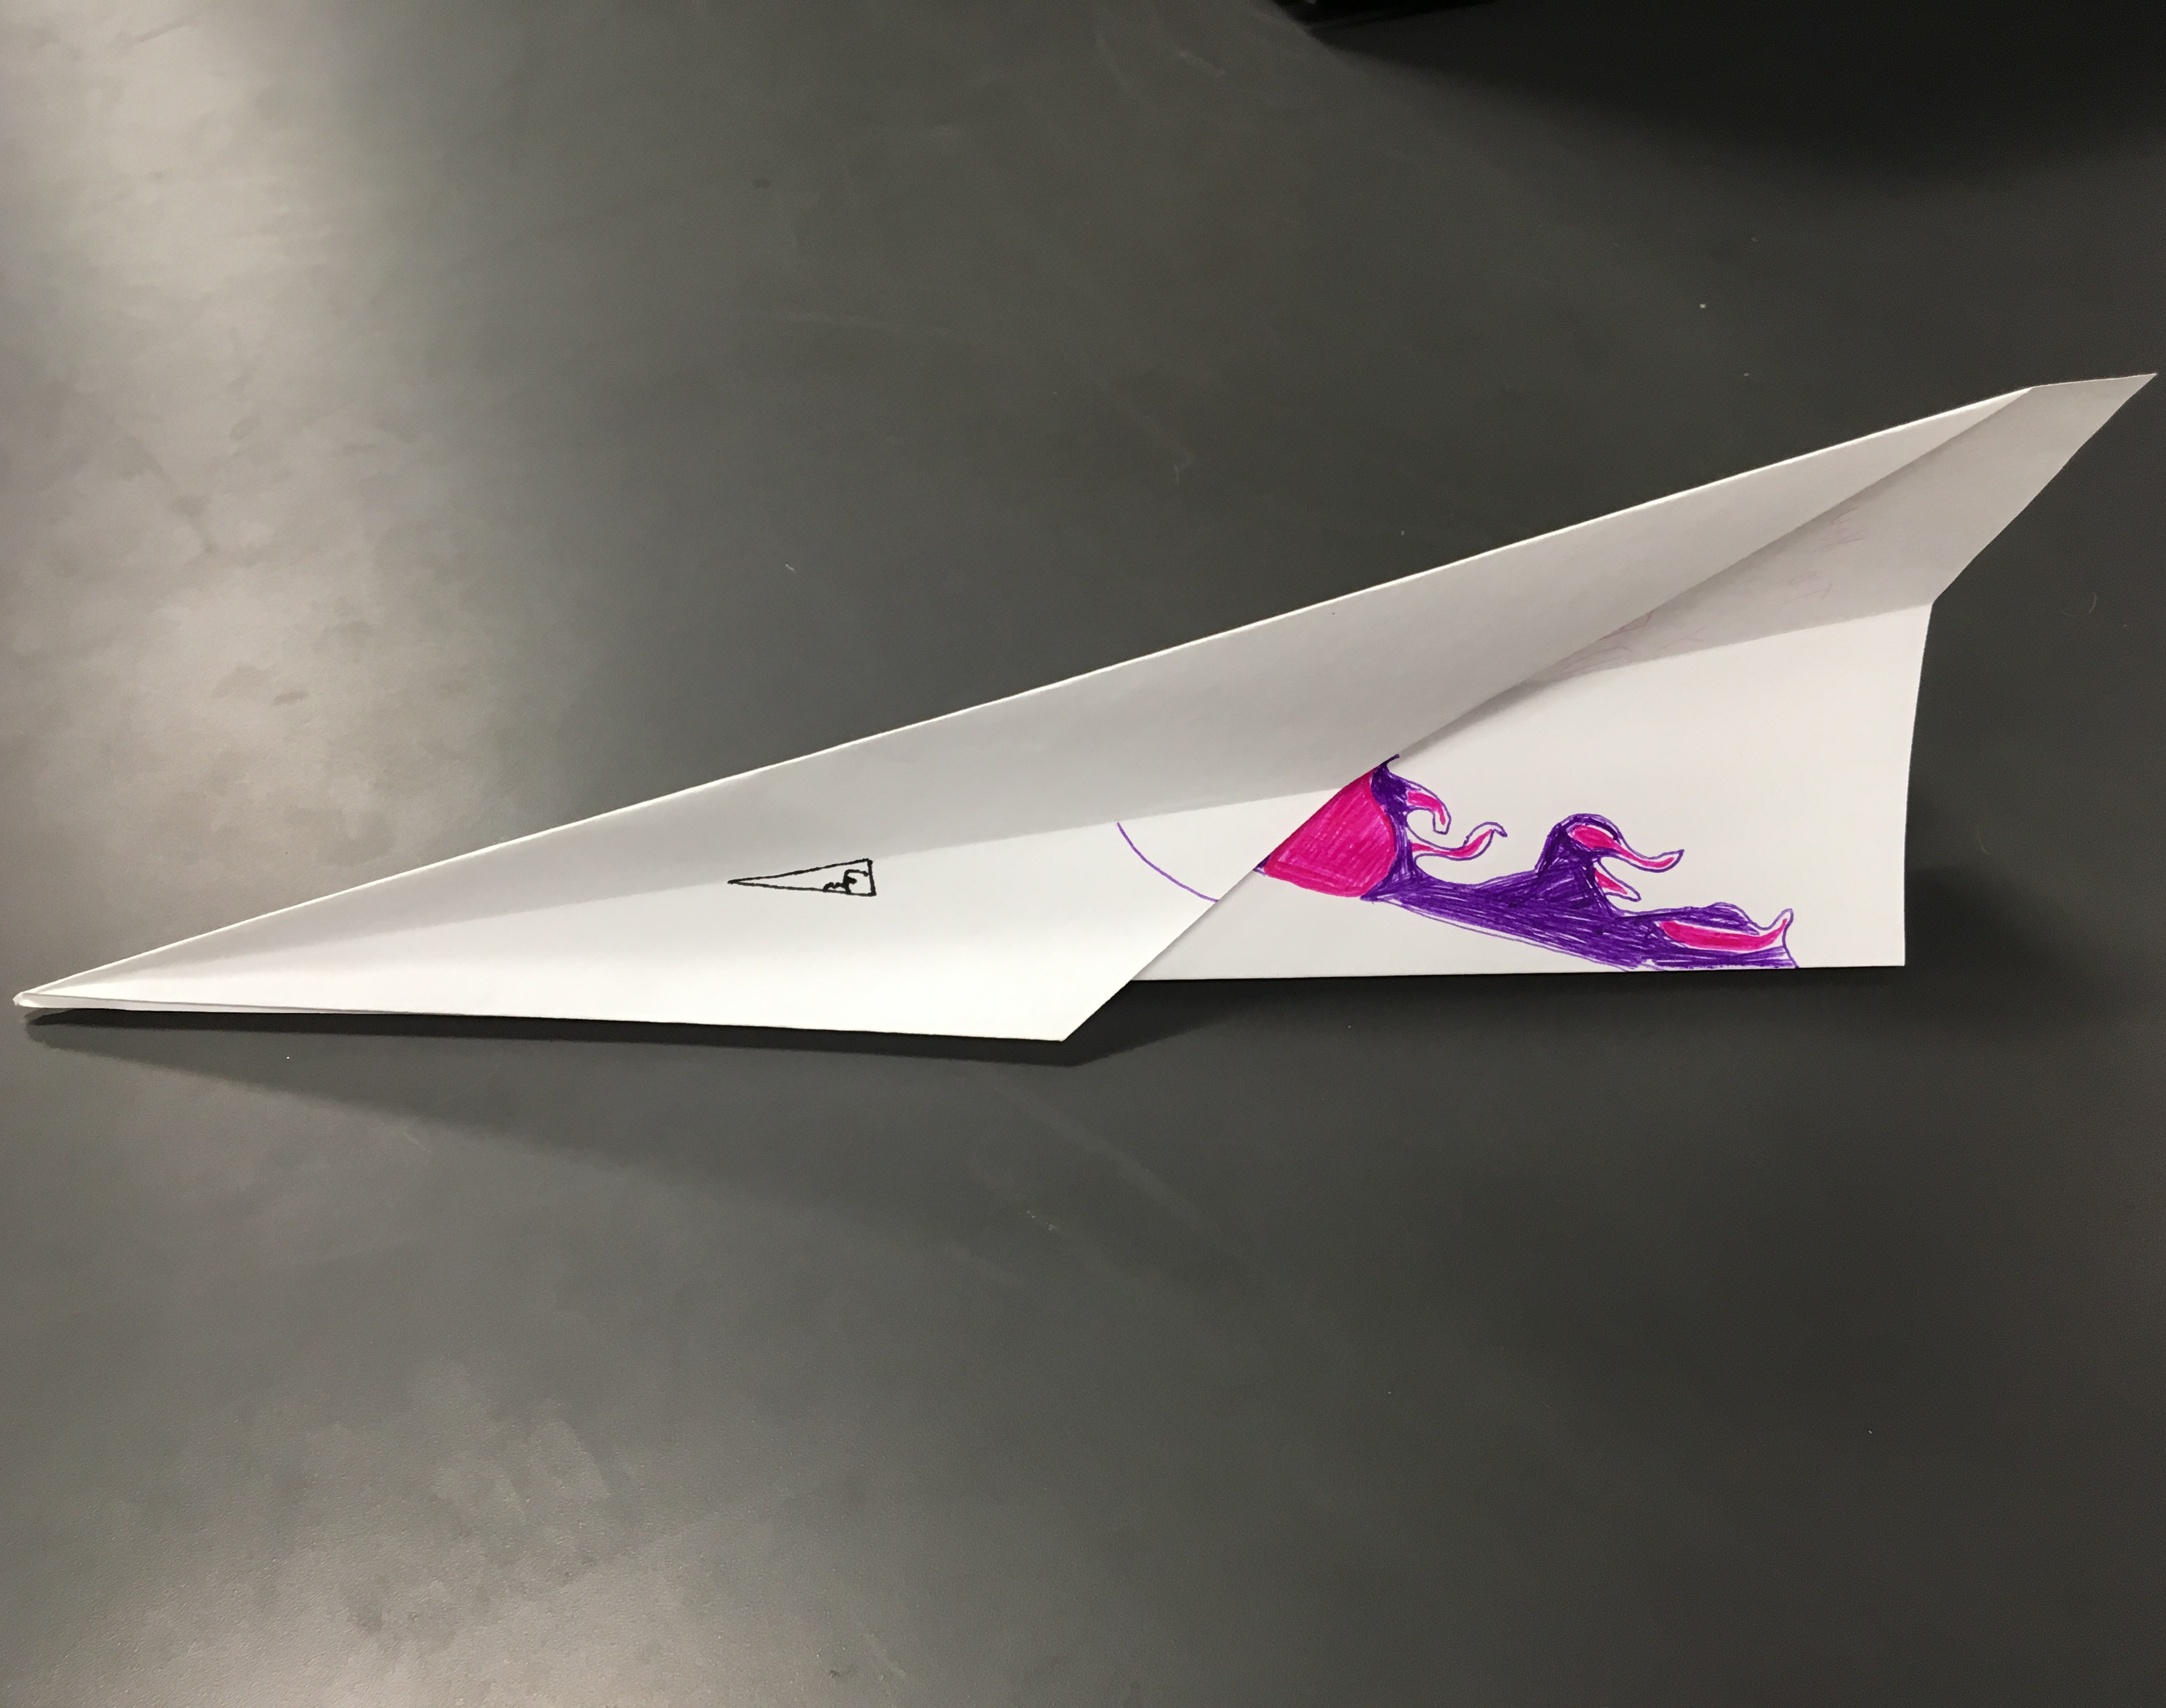
\includegraphics[width=.4\textwidth]{engl314/instructional/images/fourteenth.jpg} }}
\end{figure}

\begin{figure}[!t]
  \centering
  \caption{Throw gently release when the plane is level with the ground.}
  \subfloat{{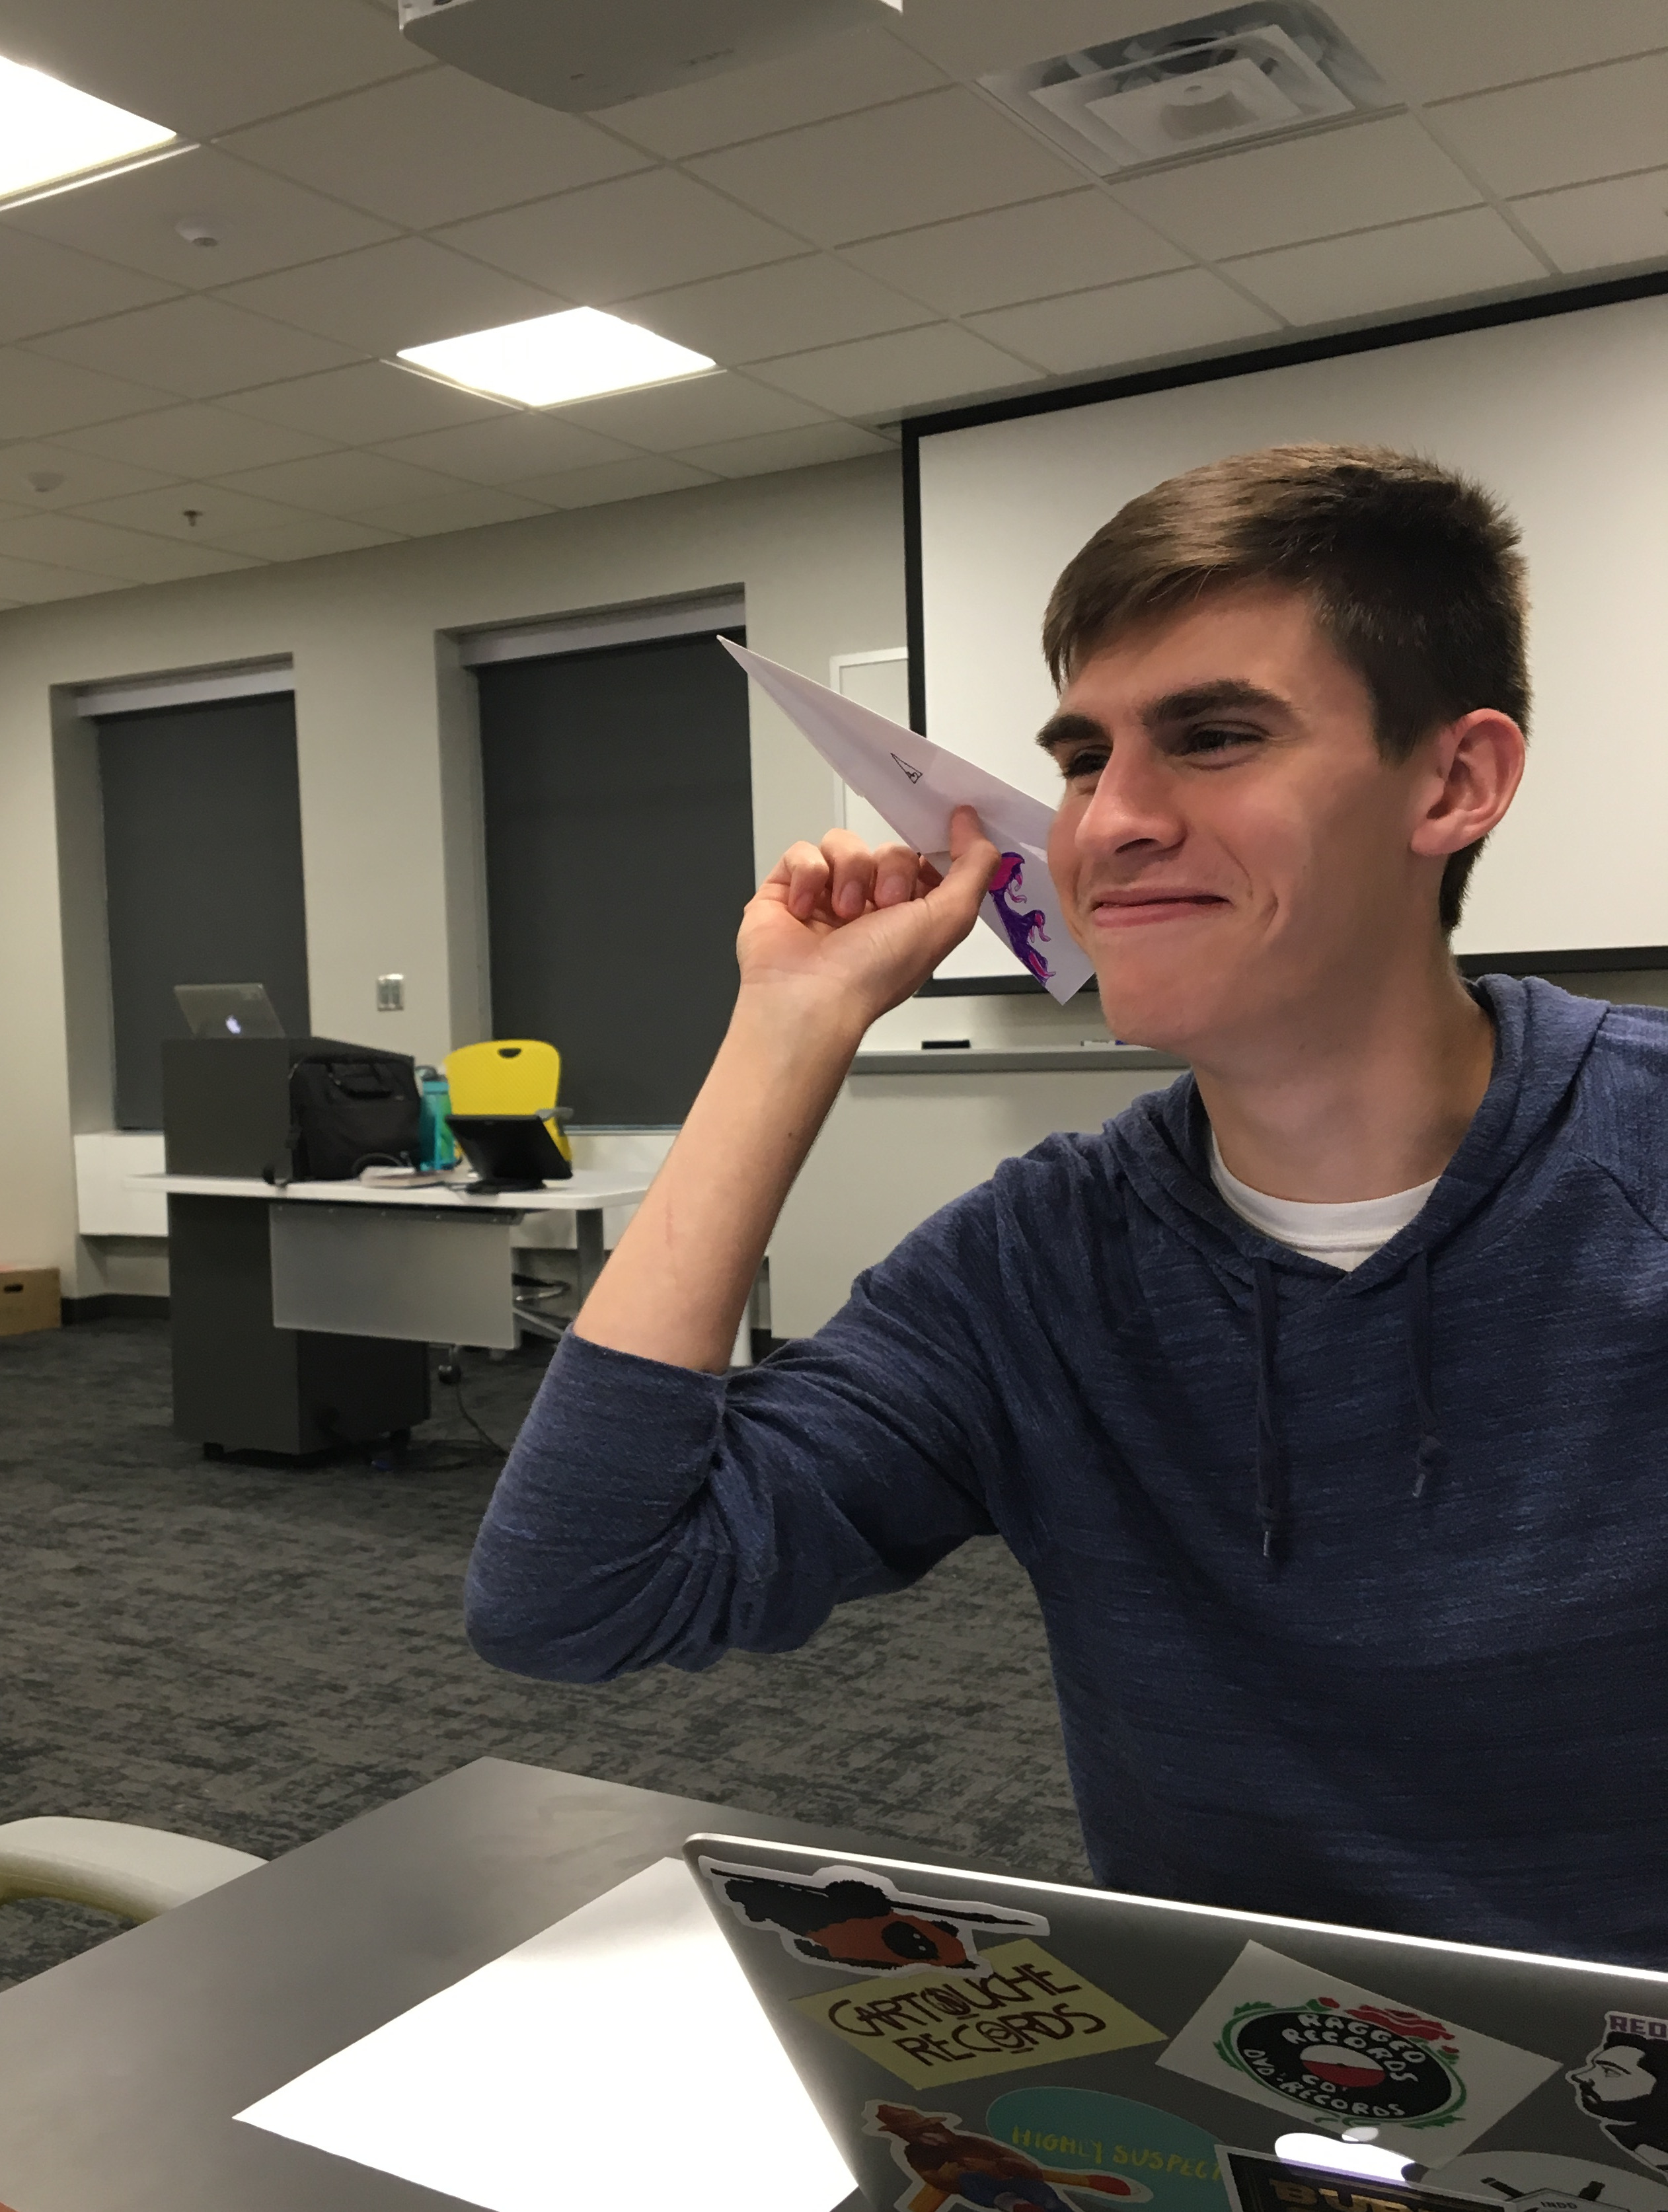
\includegraphics[width=0.4\textwidth]{engl314/instructional/images/fifteenth.jpg} }}
  \qquad
  \subfloat{{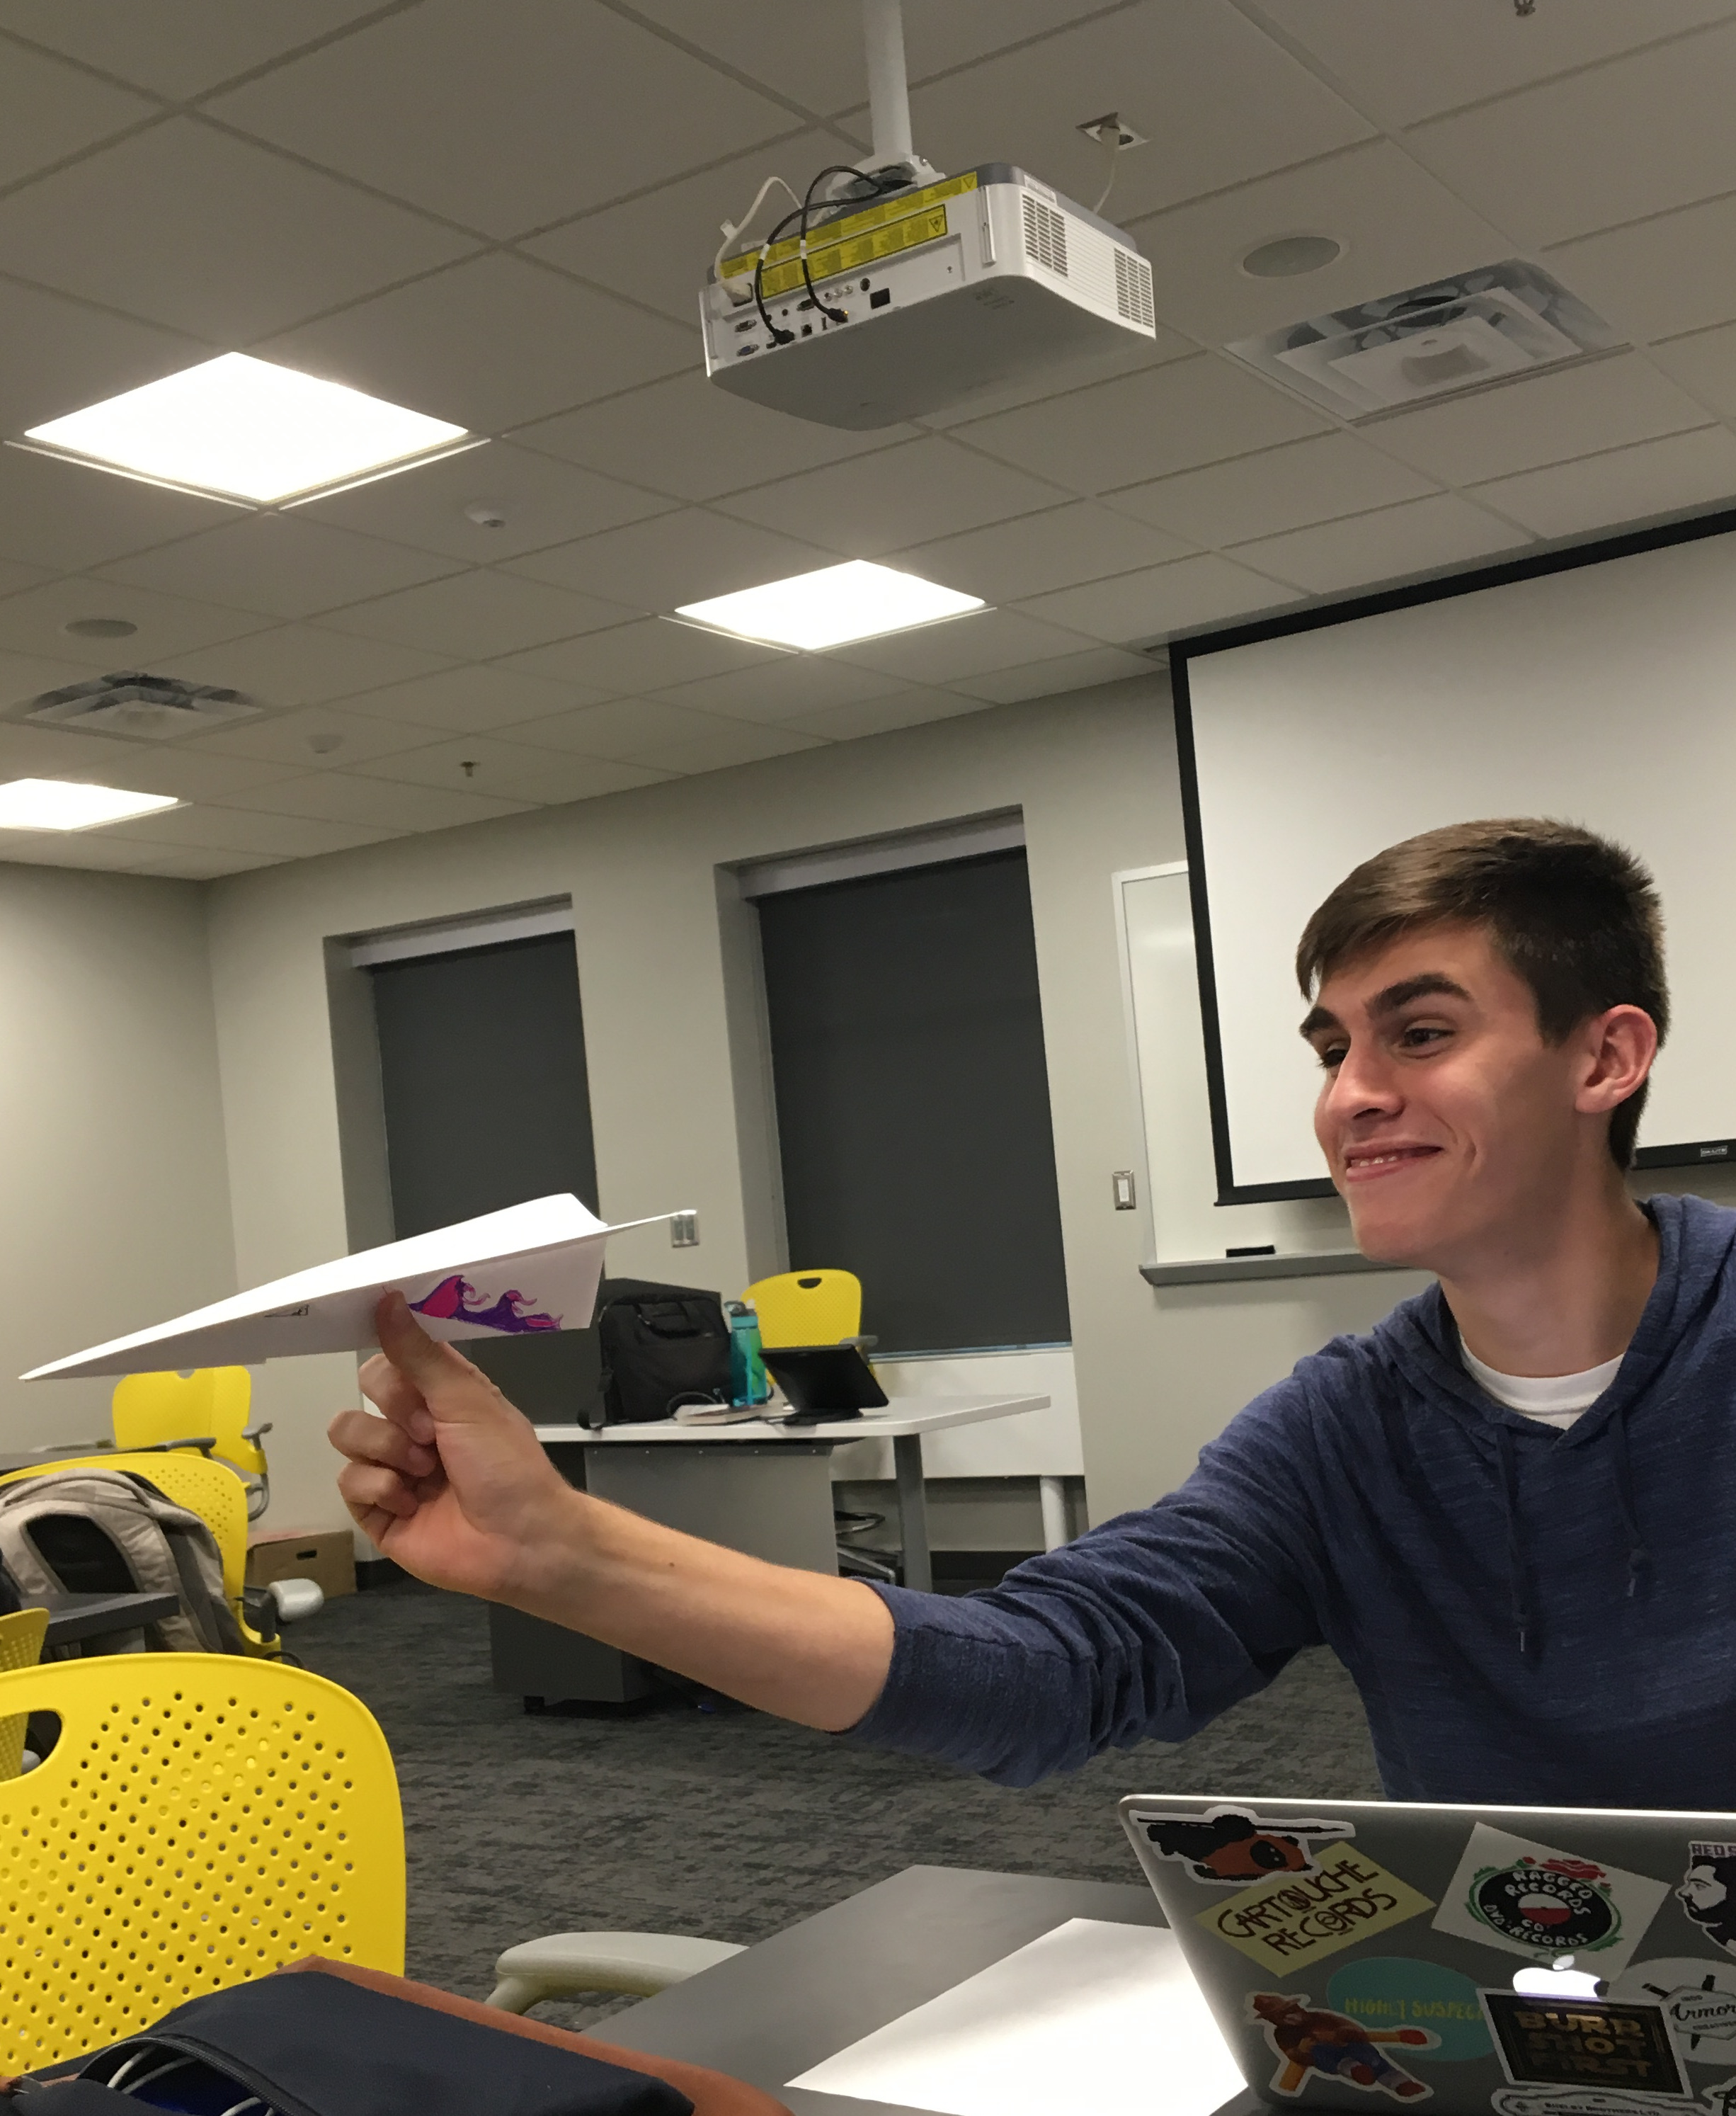
\includegraphics[width=.4\textwidth]{engl314/instructional/images/sixteenth.jpg} }}
\end{figure}

\vspace{\baselineskip}

\head{Conclusion}
\indent You have now successfully created your a paper airplane, If it did not turn out how you planned grab a new sheet and try again or add more flames.
 Have fun with your plane and be sure not to aim at any one's head
 \footnote[2]{Do not throw paper airplanes at other people, you will shoot your eye out.}
 , unless you are having a war. In that case stock up on planes and build a fort. 
 %\center
\includegraphics[width=0.4\textwidth]{engl314/instructional/images/seventeenth.jpg}

\end{document}
